\lecture{继承与派生}{lec:chap05}
\section[概念]{继承与派生的概念}\label{sec:chap05-sec01}
%%%%%%%%%%%%%%%%%%%%%%%%%%%%%% 组合、聚合和关联 %%%%%%%%%%%%%%%%%%%%%%%%%%%%%%%%%%
\begin{frame}[t, fragile]{类之间的关系}{\alert{has-a}关系---组合与聚合}%
  \begin{itemize}
  \item 组合---composition(整体与部分的关系)\\
    \begin{center}
      \begin{tikzpicture}[font=\tiny, show background grid]
        \tikzset{ coord/.style={coordinate} }
                        
        \begin{class}[text width=0.5cm ]{Car}{0, 0}
        \end{class}
                        
        \begin{class}[text width=0.5cm ]{Wheel}{3.5, -1}
        \end{class}
                        
        \begin{class}[text width=0.5cm ]{Engine}{3.5, 1}
        \end{class}
                        
        \composition{Car}{wheels}{4}{Wheel}
        \composition{Car}{Engine}{1}{Engine}
                        
      \end{tikzpicture}
    \end{center}
  \item 聚合---aggregation(松散关系)\\
    \begin{center}
      \begin{tikzpicture}[font=\tiny, show background grid]
        \tikzset{ coord/.style={coordinate} }
                        
        \begin{class}[text width=0.5cm ]{Network}{0,0}
        \end{class}
                        
        \begin{class}[text width=0.5cm ]{Computer}{3.5,0}
        \end{class}
                        
        \aggregation{Network}{1..*}{}{Computer}
                        
      \end{tikzpicture}
    \end{center}
  \end{itemize}
\end{frame}

\begin{frame}[t, fragile]{类之间的关系}{\alert{has-a}关系---复合}%
  \begin{itemize}
  \item 复合关系\\
    \begin{center}
      \begin{tikzpicture}[font=\tiny, show background grid]
        \tikzset{ coord/.style={coordinate} }
                        
        \begin{class}[text width=3cm ]{Email}{0, 0}
          \attribute{-title : string}
                        
          \operation{+edit()}
          \operation{+send(receiverAddr : string)}
          \operation{+save()} \operation{+addAttach(a
          : Attachment*)}
        \end{class}
                        
        \begin{class}[text width=2.cm ]{MailBody}{4.5,
          0}
        \end{class}
                        
        \begin{class}[text width=2.cm ]{Attachment}{4.5, -2}
          \attribute{-filename : string}
        \end{class}
                        
        \composition{Email}{1}{}{MailBody}
        \aggregation{Email}{0..*}{}{Attachment}
                        
      \end{tikzpicture}
    \end{center}
  \end{itemize}
\end{frame}

\begin{frame}[t, fragile]{类之间的关系}{\alert{has-a}关系---拥有}%
  \begin{itemize}
  \item 拥有关系\\
    \begin{center}
      \begin{tikzpicture}[font=\tiny, show background grid]
        \tikzset{ coord/.style={coordinate} }
                        
        \begin{class}[text width=1cm]{Student}{-1.7,0}
                        
        \end{class}
                        
        \begin{class}[text width=1cm]{Course}{1.7,0}
                        
        \end{class}
                                                                        
        \association{Student}{}{}{Course}{}{}{takes}
                        
        \begin{class}[text width=1cm]{Client}{-2.5,-2}
                        
        \end{class}
                        
        \begin{class}[text width=1cm]{BankAccount}{2.5,-2}
                        
        \end{class}
                        
        % 为能够在关系连线下添加表示关系的动词,
        % 对pgf-umlcd.sty的\association命令进行了个性,
        % 增加了一个参数
        \association{BankAccount}{1..5}{-accounts}{Client}{1}{+owner}{has}
                        
      \end{tikzpicture}
    \end{center}
  \end{itemize}
\end{frame}

\begin{frame}[t, fragile]{类之间的关系}{\alert{is-a}---继承与派生}%
  \begin{itemize}
  \item 继承与派生类\\
    \begin{center}
      \begin{tikzpicture}[font=\tiny, show background grid]
        \tikzset{ coord/.style={coordinate} }
                        
        \begin{class}[text width=1.5cm ]{GrandFather}{0 ,0}
        \end{class}                        

        \begin{class}[text width=1.5cm ]{Father}{0, -1.5}
          \inherit{GrandFather}
        \end{class}

        \begin{class}[text width=1.5cm ]{Son}{0, -3.0}
          \inherit{Father}
        \end{class}
      \end{tikzpicture}
    \end{center}
  \end{itemize}
\end{frame}
%%%%%%%%%%%%%%%%%%%%%%%%%%%%%% 继承与派生的概念 %%%%%%%%%%%%%%%%%%%%%%%%%%%%%%%%%%
\begin{frame}[t, fragile]{继承与派生}{基本概念}%
  \stretchon
  \begin{itemize}
  \item 用已有类定义新类,新类拥有原有类的全部特征
    \begin{itemize}
    \item 原有类$\Rightarrow$\alert{基类(父类)}
    \item 新类$\Rightarrow$\alert{派生类}
    \end{itemize}
  \item 可以\alert{多继承}(一个派生类有多个基类)和\alert{多层派
      生}(多层继承)
  \item 特点:新类可以\alert{继承}原有类的属性和行为,并且可以
    \alert{添加}新的属性和行为,或更新原有类的成员
  \item 优点:\alert{代码重用}
  \end{itemize}
  \stretchoff
\end{frame}

\begin{frame}[t, fragile]{继承与派生}{应用实例}%
  \begin{itemize}
  \item 例子:C++输入输出流类\\
    \begin{center}
      \begin{tikzpicture}[font=\tiny, show background grid]
        \tikzset{ coord/.style={coordinate} }
        
        \begin{class}[scale=0.6,text width=0.5cm ]{ios}{0 ,0}          
        \end{class}

        \begin{class}[scale=0.6,text width=0.5cm ]{istream}{-1.0, -1.5}
          \inherit{ios}
        \end{class}

        \begin{class}[scale=0.6,text width=0.5cm ]{ostream}{1.0, -1.5}
          \inherit{ios}
        \end{class}

        \begin{class}[scale=0.6,text width=0.5cm ]{ifstream}{-2.0, -3.0}
          \inherit{istream}
        \end{class}

        \begin{class}[scale=0.6,text width=0.5cm ]{iostream}{0.0, -3.0}
          \inherit{istream}
          \inherit{ostream}
        \end{class}

        \begin{class}[scale=0.6,text width=0.5cm ]{ofstream}{2.0, -3.0}
          \inherit{ostream}
        \end{class}

        \begin{class}[scale=0.6,text width=0.5cm ]{fstream}{0.0, -4.5}
          \inherit{iostream}
        \end{class}

        \umlnote[scale=0.6,text width=1.2cm, left=of
        ifstream](note1) {Defined in fsteam.h};
        \umlnote[scale=0.6,text width=1.2cm, right=of
        ofstream](note2) {Defined in fsteam.h};

        \draw[red, dashed, thick](note1) -- (ifstream);
        \draw[red, dashed, thick](note2) -- (ofstream);
      \end{tikzpicture}
    \end{center}    
  \end{itemize}
\end{frame}

\begin{frame}[t, fragile]{继承与派生}{应用实例}%
  \begin{itemize}
  \item 例子:MFC类层次
  \end{itemize}
  \begin{center}
    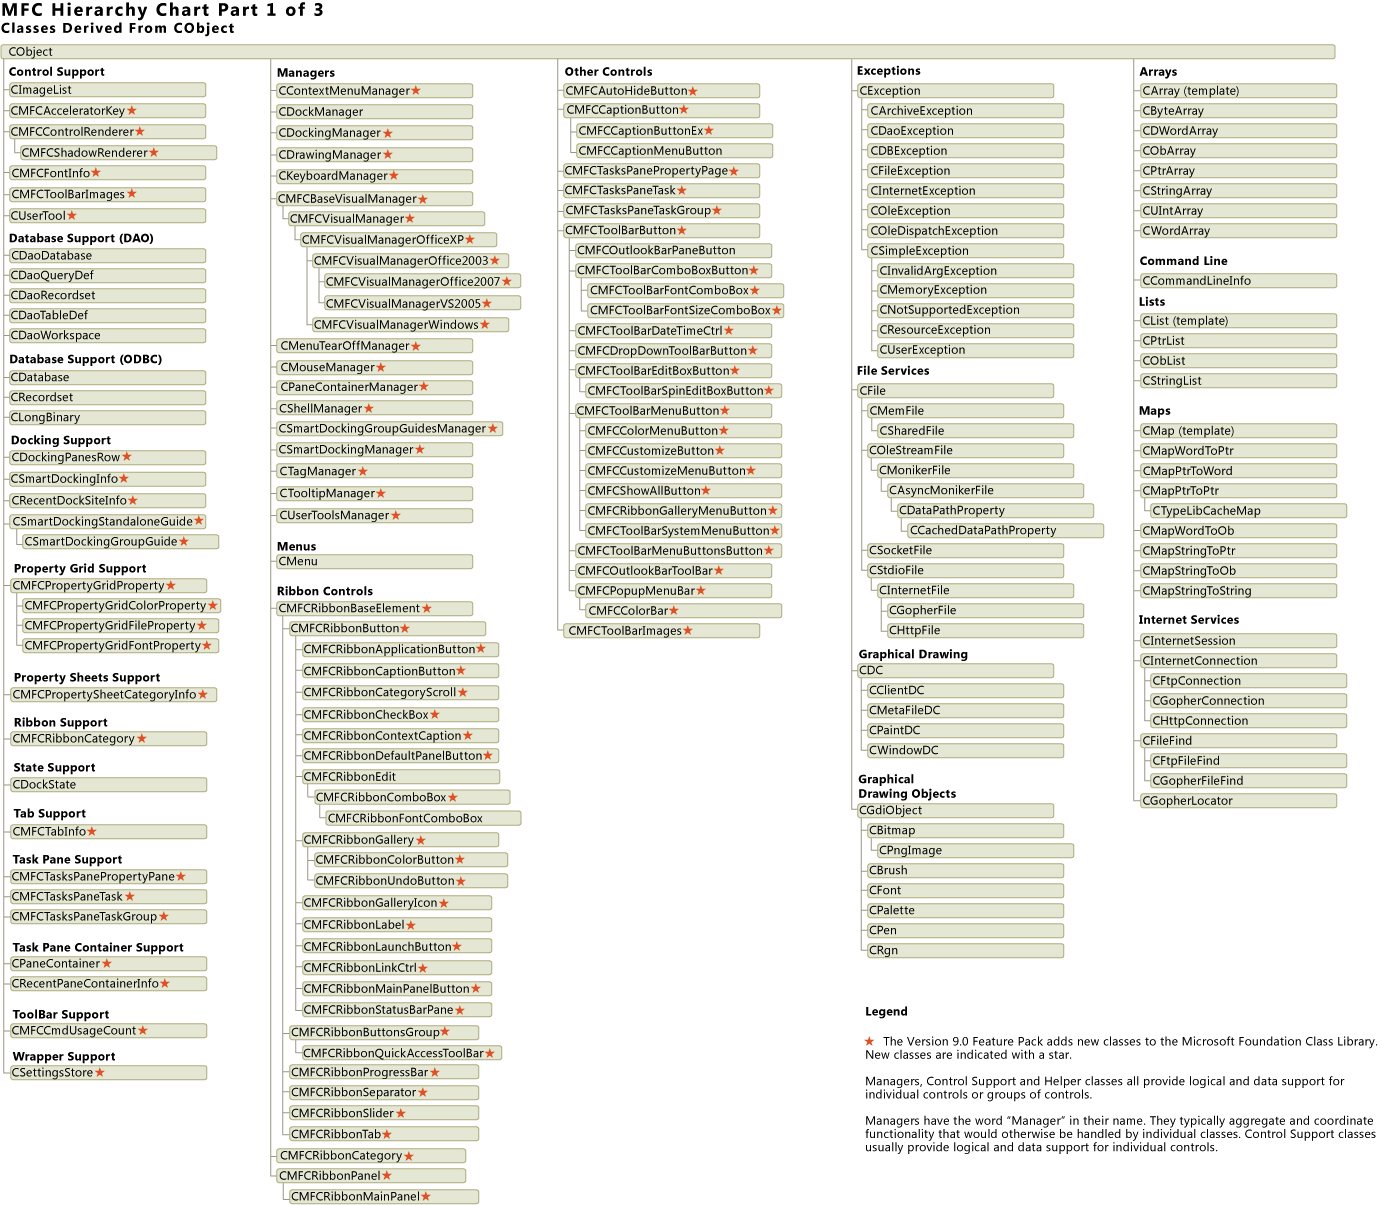
\includegraphics[height=0.7\textheight]{chap05/01MFC01}
  \end{center}
\end{frame}

\begin{frame}[t, fragile]{继承与派生}{应用实例}%
  \begin{itemize}
  \item 例子:MFC类层次
  \end{itemize}
  \begin{center}
    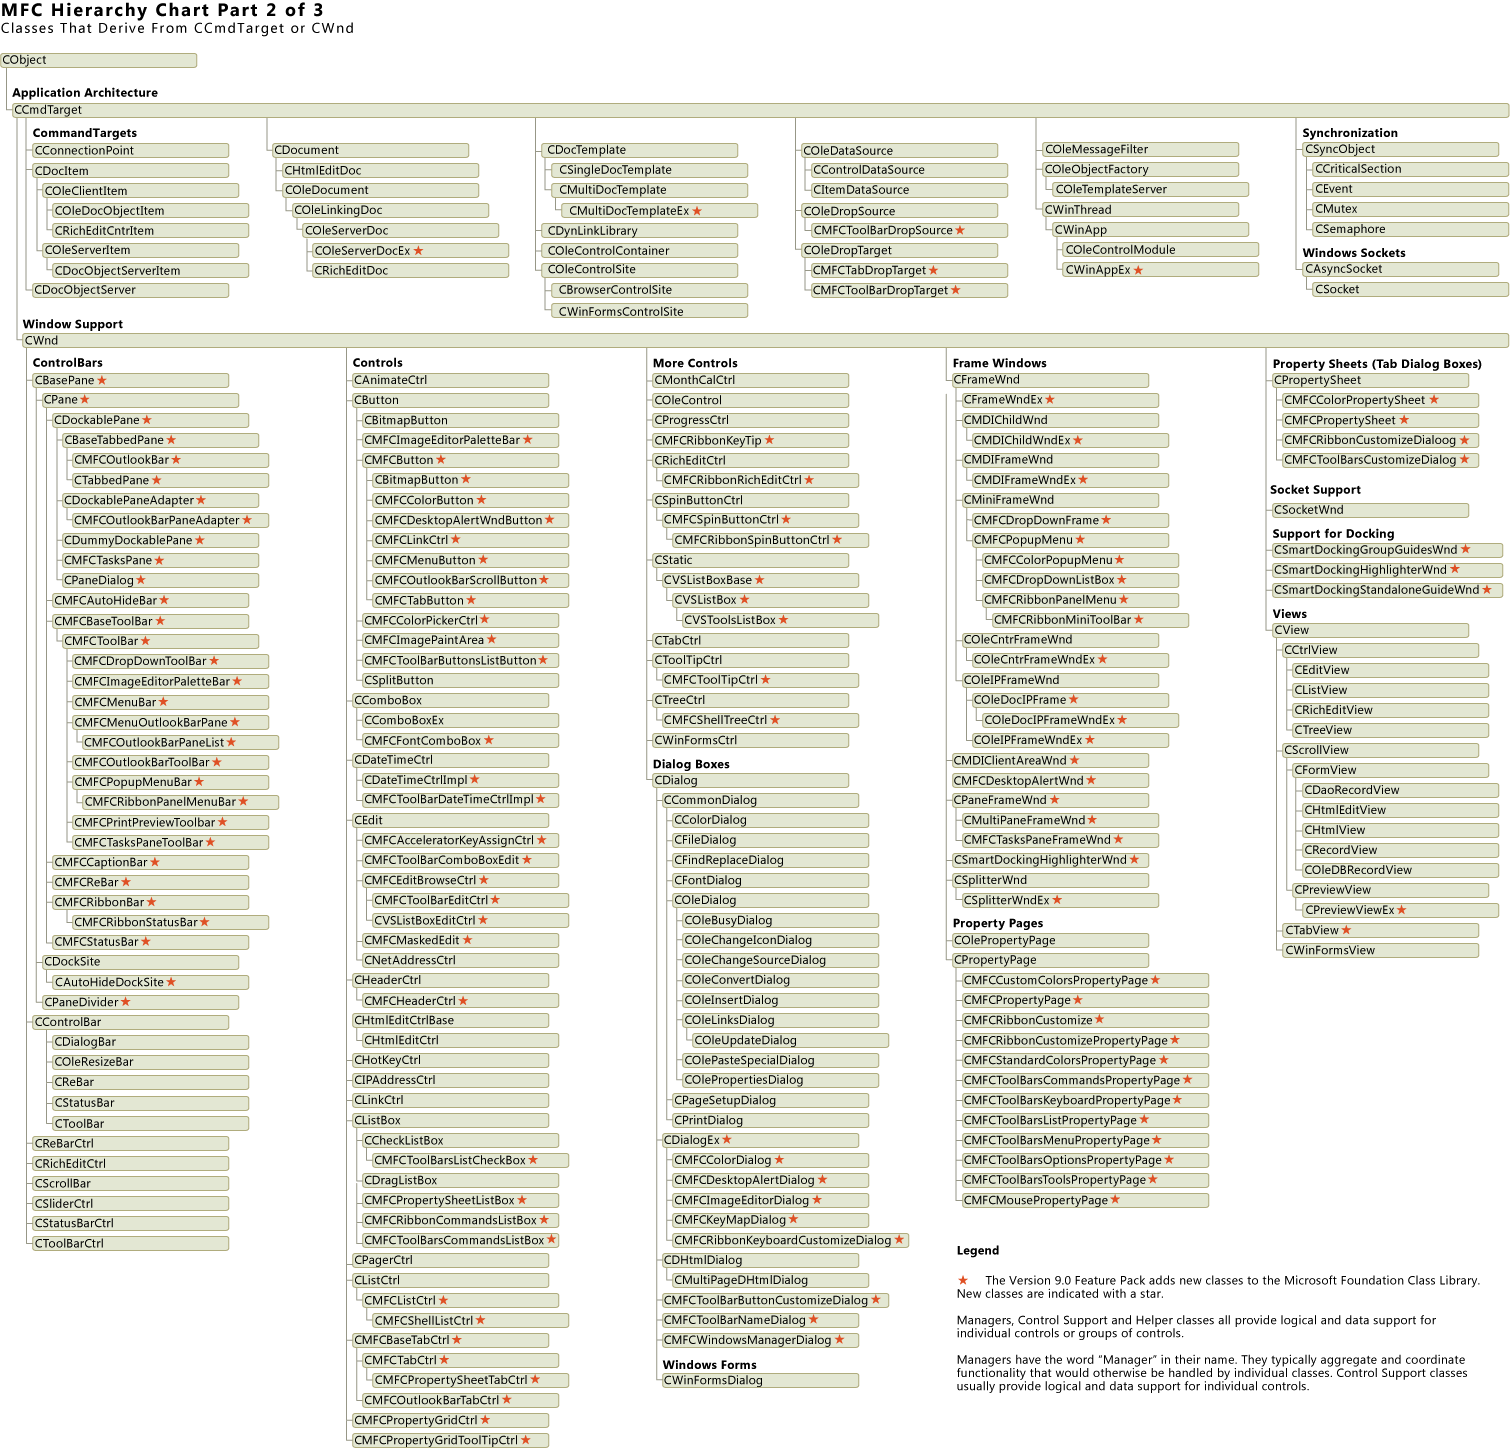
\includegraphics[height=0.7\textheight]{chap05/01MFC02}
  \end{center}
\end{frame}

\begin{frame}[t, fragile]{继承与派生}{应用实例}%
  \begin{itemize}
  \item 例子:MFC类层次
  \end{itemize}
  \begin{center}
    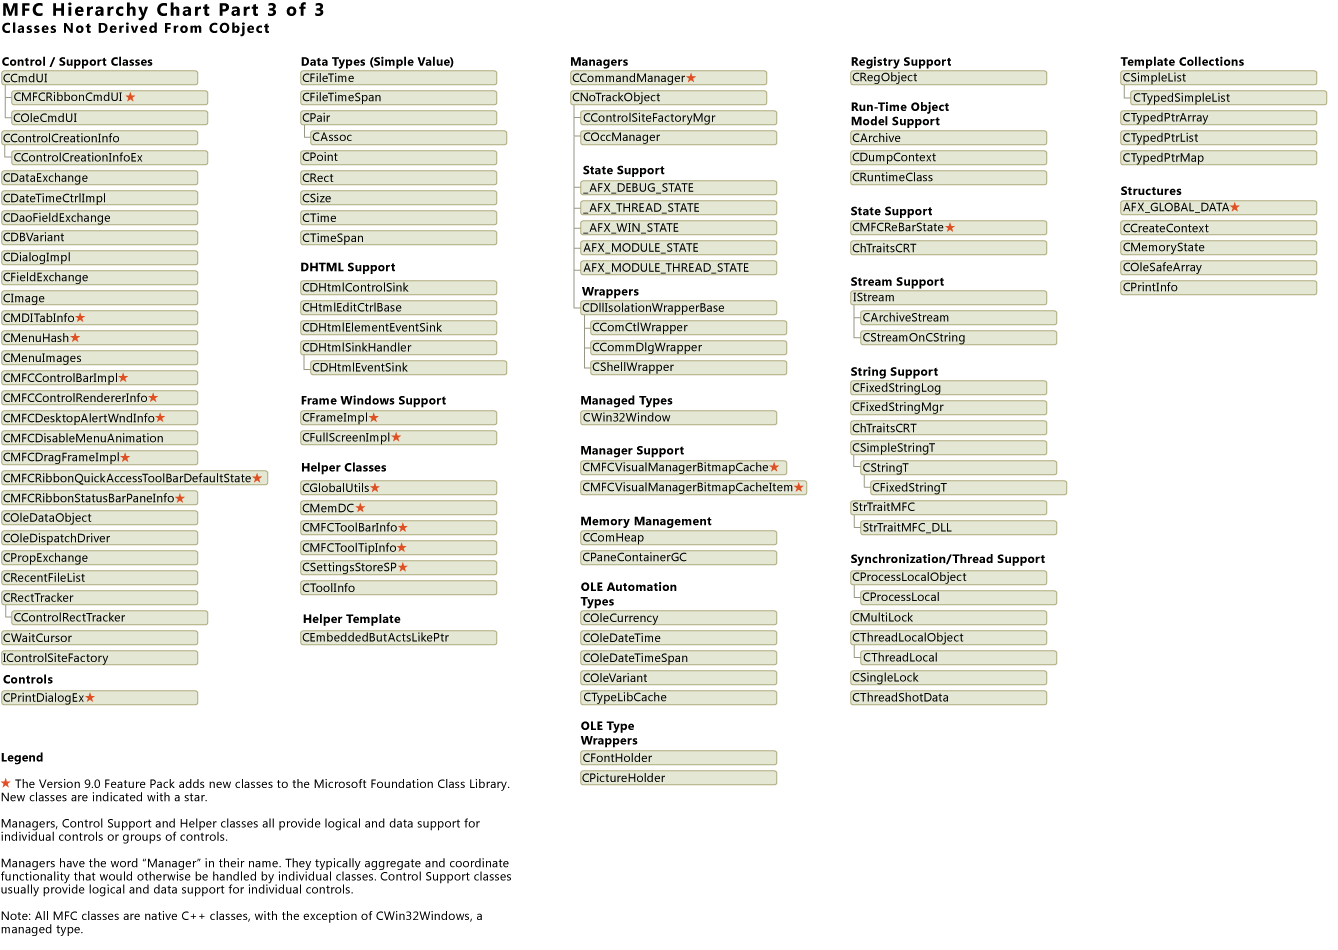
\includegraphics[height=0.7\textheight]{chap05/01MFC03}
  \end{center}
\end{frame}

\begin{frame}[t, fragile]{继承与派生}{应用实例}%
  \begin{itemize}
  \item 例子:QT类层次
  \end{itemize}
  \begin{center}
    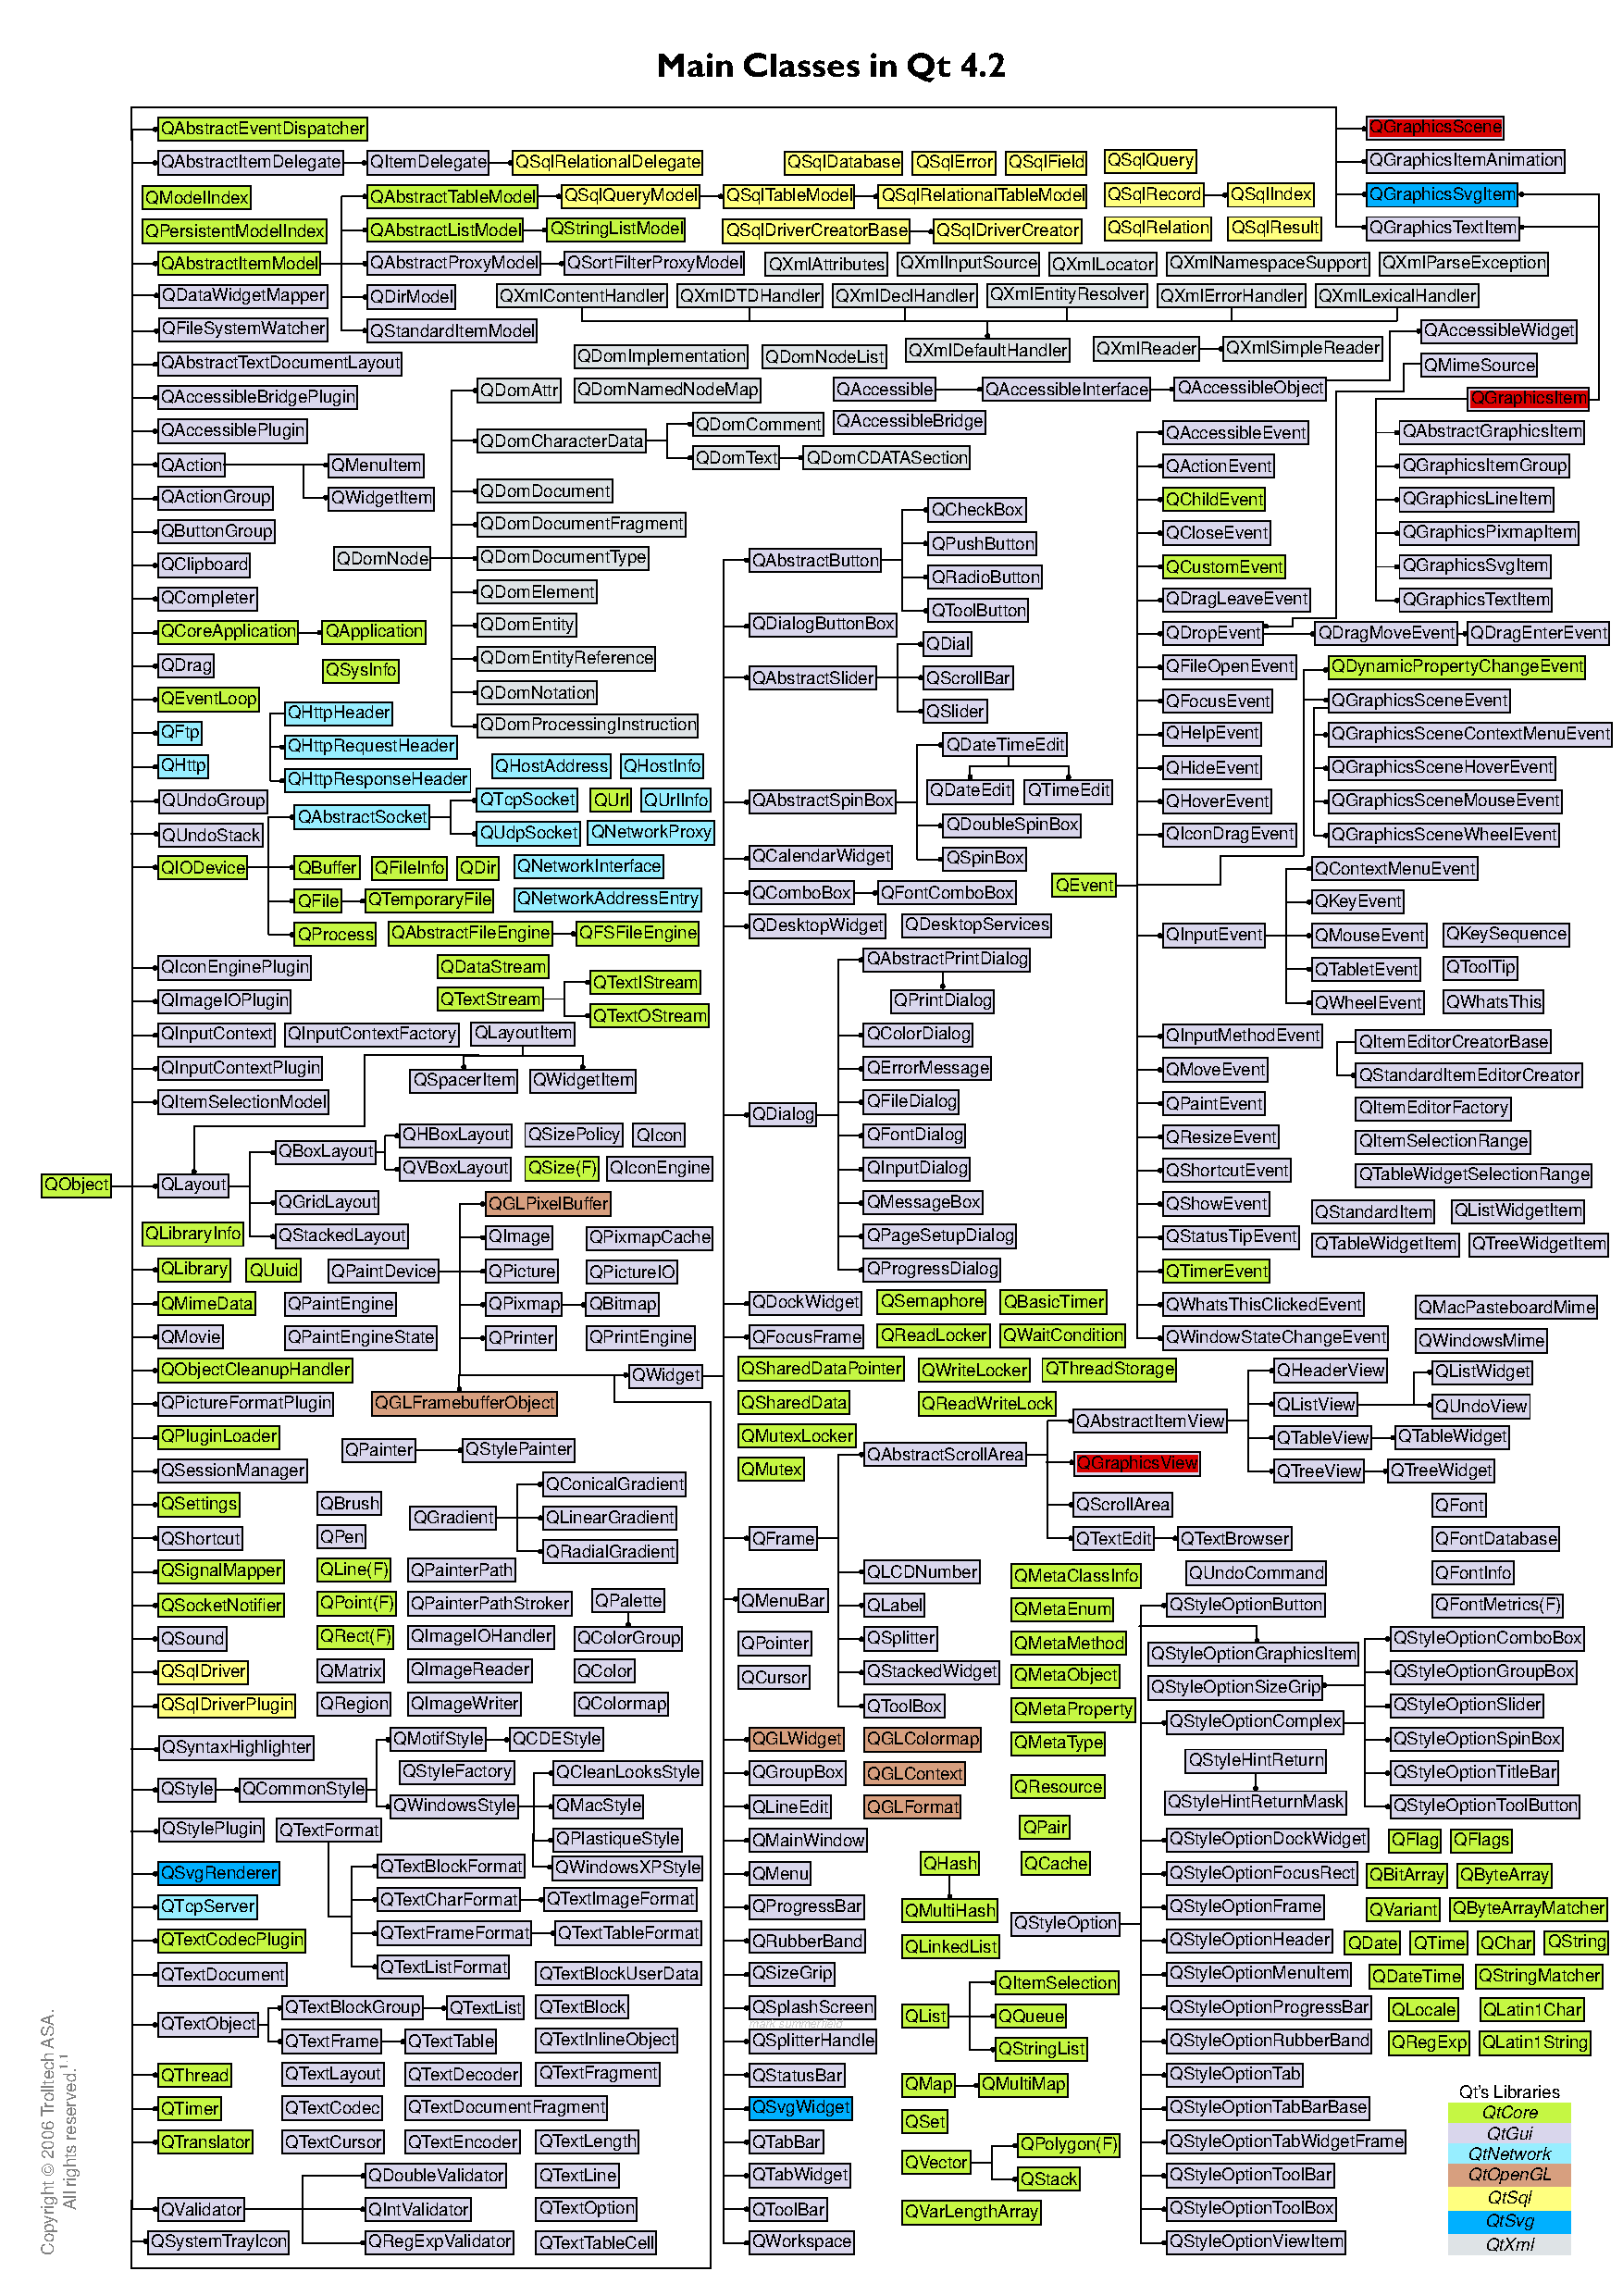
\includegraphics[height=0.7\textheight]{chap05/02qt42}
  \end{center}
\end{frame}

\begin{frame}[t, fragile]{继承与派生}{基本语法}%
  \begin{itemize}
  \item 派生类的定义
  \end{itemize}
  \begin{center}
    \begin{tikzpicture}[font=\tiny, show background grid]
      \tikzset{ coord/.style={coordinate} }
      \umlnote[text width=0.4\textwidth](note1) at (0, 0)
      {
        \begin{cppttnobg}
class |派生类名|: |继承方式|1 |基类名|1,
        |继承方式|2 |基类名|2, |$\cdots$|
{
private:
  |派生类的私有数据和函数|;
public:
  |派生类的公有数据和函数|;
protected:
  |派生类的保护数据和函数|;
};
        \end{cppttnobg}
      };

      \umlnote[text width=0.3\textwidth](note1) at (4, -1)
      {
        继承方式:    
        \begin{cppttnobg}          
public:       |公有继承|
private:     |私有继承|
protected:  |保护继承|          
        \end{cppttnobg}
      };      
    \end{tikzpicture}
  \end{center}
\end{frame}

\begin{frame}[t, fragile]{继承与派生}{形状类实例分析}%
  \begin{itemize}
  \item 用继承方式实现基本形状类
  \end{itemize}
  \begin{center}
    \begin{tikzpicture}[font=\tiny, show background grid]
      \tikzset
      {
        coord/.style={coordinate},
        cube/.style={black}
      }
      
      \node[anchor=west] (drawbox) at (-1,-1)
      {
        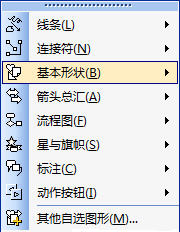
\includegraphics[width=0.2\textwidth]{chap05/03-01drawbox}
      };

      \path let \p{d}=(drawbox) in
      coordinate (f00) at (\x{d}, \y{d})
      coordinate (f11) at ($(f00) + (0.9, 1.0)$)
      coordinate (f12) at ($(f00) + (0.9, 0.57)$)
      ;
      \fill[red](f11)circle[radius=1pt];
      \fill[red](f12)circle[radius=1pt];      

      \node[anchor=west] (linebox) at (1,1)
      {
        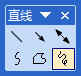
\includegraphics[width=0.08\textwidth]{chap05/03-02linebox}
      };

      \node[anchor=west] (shapebox) at (2,-1)
      {
        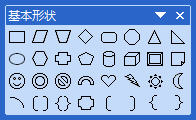
\includegraphics[width=0.2\textwidth]{chap05/03-03shapebox}
      };

      \path let \p{s}=(shapebox) in
      coordinate (s00) at (\x{s}, \y{s})
      coordinate (s11) at ($(s00) + (-1.08, 0.28)$)
      coordinate (s12) at ($(s00) + (-1.08, 0.02)$)
      coordinate (s13) at ($(s00) + (0.76, 0.24)$);
      \fill[red](s11)circle[radius=1pt];
      \fill[red](s12)circle[radius=1pt];
      \fill[red](s13)circle[radius=1pt];

      \draw [-{Stealth[scale=1.0]}, red, thick] (f11.north)
      to[out=0,in=-90] (linebox.south);
      \draw [-{Stealth[scale=1.0]}, red, thick] (f12.east)
      to[out=0,in=180] (shapebox.west);
      

      \node[fill=blue!25, rectangle, draw, right=of linebox](rect)
      {CRectangle};
      \node[fill=blue!25, ellipse, draw, below=of shapebox,
      xshift=-0.7cm, yshift=0.7cm](ellip)
      {CEllipse};

      \draw [-{Stealth[scale=1.0]}, red, thick] (s11.north)
      to[out=90,in=180] (rect.west);
      \draw [-{Stealth[scale=1.0]}, red, thick] (s12.south)
      to[out=-90,in=90] (ellip.north);
      
      \node[coord, below=of shapebox, xshift=2cm] (donut1) {};
      \draw[fill=blue!25] (donut1) circle [radius=1];
      \node[fill=white, circle, draw](donut) at (donut1)  {CDonut};

      \draw [-{Stealth[scale=1.0]}, red, thick] (ellip.east)
      to[out=0,in=180] (donut.west);

      \node[coord, right=of shapebox] (tri) {};
      \path let \p{t00}=(tri) in
      coordinate (t1) at (\x{t00}, \y{t00})
      coordinate (t2) at ($(t1) + (1, 1)$)
      coordinate (t3) at ($(t2) + (1, -1)$)
      coordinate (t4) at ($(t1)!0.5!(t3)$)
      coordinate (tc) at ($(t2)!0.5!(t4)$);
      \draw[fill=blue!25] (t1) -- (t2) -- (t3) -- cycle;            
      \node(triangle) at ($(tc)+(0,-0.2)$) {CTriangle};

      \draw [-{Stealth[scale=1.0]}, red, thick] (s13.east)
      to[out=0,in=180] (triangle.west);

      % draw the top and bottom of the cube
      \node[coord, right=of rect] (cubestart) {};

      \path let \p{c00}=(cubestart) in
      coordinate (c11) at (\x{c00}, \y{c00})
      coordinate (c12) at ($(c11) + (0, 1, 0)$)
      coordinate (c13) at ($(c11) + (1, 1, 0)$)
      coordinate (c14) at ($(c11) + (1, 0, 0)$)
      coordinate (c21) at ($(c11) + (0, 0, 1)$)
      coordinate (c22) at ($(c11) + (0, 1, 1)$)
      coordinate (c23) at ($(c11) + (1, 1, 1)$)
      coordinate (c24) at ($(c11) + (1, 0, 1)$);

      % draw the edges of the cube
      \draw[cube] (c11) -- (c21);
      \draw[cube] (c12) -- (c22);
      \draw[cube] (c13) -- (c23);
      \draw[cube] (c14) -- (c24);
   
      \draw (c11) -- (c12) -- (c13) -- (c14) -- cycle;
      \draw[fill=blue!25] (c21) -- (c22) -- (c23) -- (c24) -- cycle;
      \draw[fill=blue!25] (c22) -- (c12) -- (c13) -- (c23) -- cycle;
      \draw[fill=blue!25] (c24) -- (c23) -- (c13) -- (c14) -- cycle;

      \node(cube) at ($ (c22) !.5! (c24) $) {CCuboid};

      \draw [-{Stealth[scale=1.0]}, red, thick] (rect.east)
      to[out=0,in=180] (cube.west);      
    \end{tikzpicture}
  \end{center}
\end{frame}

\begin{frame}[t, fragile]{继承与派生}{形状类实例分析}%
  \begin{itemize}
  \item 基类:形状类(CShape)
  \end{itemize}
  \begin{center}
    \begin{tikzpicture}[font=\tiny, show background grid]
      \tikzset{ coord/.style={coordinate} }

      \begin{class}[fill=green!25, text width=3em]{形状类CShape}{0 ,0}
      \end{class}

      \begin{class}[fill=blue!25, text width=5em]{等腰三角形类 CTriangle}{-3.0, -2.0}
        \inherit{形状类CShape}
      \end{class}

      \begin{class}[fill=green!25, text width=3em]{矩形类CRectangle}{0.0, -2.0}
        \inherit{形状类CShape}
      \end{class}

      \begin{class}[fill=green!25, text width=3em]{椭圆类CEllipse}{3.0, -2.0}
        \inherit{形状类CShape}
      \end{class}

      \begin{class}[fill=blue!25, text width=4em]{长方体类CCuboid}{0.0, -4.0}
        \inherit{矩形类CRectangle}
      \end{class}

      \begin{class}[fill=green!25, text width=3em]{圆环类CDonut}{3.0, -4.0}
        \inherit{椭圆类CEllipse}
      \end{class}
    \end{tikzpicture}
  \end{center}
\end{frame}

\begin{frame}[t, fragile]{继承与派生}{形状类实例分析}%
  \stretchon
  \begin{itemize}
  \item 用继承方式实现基本形状类
    \begin{itemize}
    \item 功能描述\\
      \begin{minipage}{0.55\linewidth}
        \begin{itemize}
        \item 带文本的基本形状绘制
        \item 可更改文本和形状的颜色
        \item 可更改形状的大小
        \item 可上下左右移动形状
        \end{itemize}
      \end{minipage}\\%\quad
      \centering
      \begin{minipage}{0.75\linewidth}
        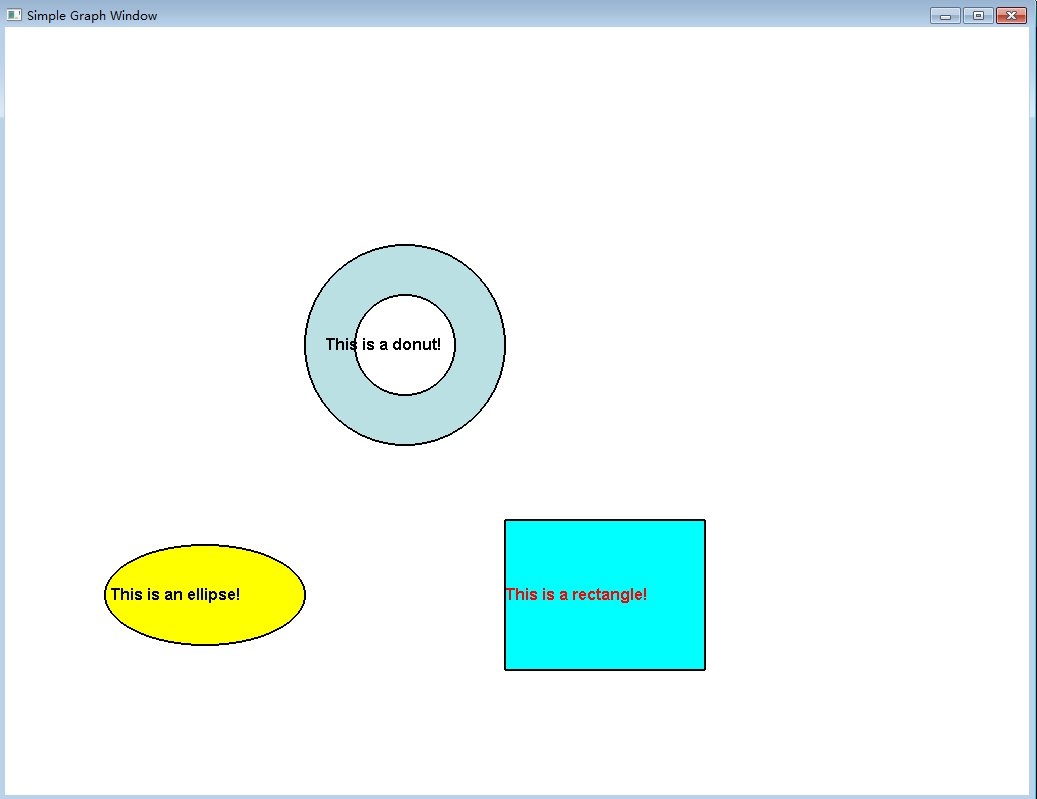
\includegraphics[width=0.65\textwidth]{chap05/04shapefig}
      \end{minipage}
    \end{itemize}
  \end{itemize}
  \stretchoff
\end{frame}

\begin{frame}[t, fragile]{继承与派生}{形状类实例分析}%
  \begin{itemize}
  \item 用继承方式实现基本形状类
  \end{itemize}
  \begin{center}
    \begin{tikzpicture}[font=\tiny, show background grid]
      \tikzset{ coord/.style={coordinate} }
      \umlnote[text width=0.45\textwidth](note1) at (0, 0)
      {
        \cppfilettnobg{codes/chap05/05-01Point2D.h}
      };

      \umlnote[text width=0.45\textwidth](note2) at (5, 0)
      {
        \cppfilettnobg{codes/chap05/05-02Shape.h}
      };
      % \node [coord](a1) at (-0.45, -2.05) {文本颜色};文本内容;全局坐标;对象颜色
      
      \path let \p1=(note2) in
      coordinate (note20) at (\x1, \y1)
      coordinate (txt) at ($(note20) + (1.2, 2.2)$)
      coordinate (tn11) at ($(note20) + (-1.10, 1.15)$)
      coordinate (tn21) at ($(note20) + (-0.95, 0.9)$)
      coordinate (tn31) at ($(note20) + (-1.32, 0.38)$)
      coordinate (tn41) at ($(note20) + (-1.22, 0.13)$)
      ;

      \node [draw,fill=blue!20](tcolor) at (txt) {文本颜色};
      \node [draw,fill=blue!20,below=0.15 of tcolor](tcontent) {文本内容};
      \node [draw,fill=blue!20,below=0.15 of tcontent](tcoord) {全局坐标};
      \node [draw,fill=blue!20,below=0.15 of tcoord](objcolor) {对象颜色};
      \node [draw,fill=blue!20,below=0.15 of note2, xshift=-0.5cm](prop)
      {所有基本形状共用数据成员};

      \node [coord,right=10pt of tcolor](tn12) {};
      \node [coord,right=10pt of tcontent](tn22) {};
      \node [coord,right=10pt of tcoord](tn32) {};
      \node [coord,right=10pt of objcolor](tn42) {};
      
      \fill[red](tn11)circle[radius=1pt];
      \fill[red](tn21)circle[radius=1pt];
      \fill[red](tn31)circle[radius=1pt];
      \fill[red](tn41)circle[radius=1pt];

      \draw [-{Stealth[scale=1.0]}, red, thick] (tn11.east)
      to[out=0,in=180] (tcolor.west);
      \draw [-{Stealth[scale=1.0]}, red, thick] (tn21.east)
      to[out=0,in=180] (tcontent.west);
      \draw [-{Stealth[scale=1.0]}, red, thick] (tn31.east)
      to[out=0,in=180] (tcoord.west);
      \draw [-{Stealth[scale=1.0]}, red, thick] (tn41.east)
      to[out=0,in=180] (objcolor.west);

      \draw [-{Stealth[scale=1.0]}, red, thick] (tcolor.east)-- (tn12)
      |- (prop.east);
      \draw [red, thick] (tcontent.east)-- (tn22);
      \draw [red, thick] (tcoord.east)-- (tn32);
      \draw [red, thick] (objcolor.east)-- (tn42);
    \end{tikzpicture}
  \end{center}
\end{frame}

\begin{frame}[t, fragile]{继承与派生}{形状类实例分析}%
  \begin{itemize}
  \item 用继承方式实现基本形状类
  \end{itemize}
  \begin{center}
    \begin{tikzpicture}[font=\tiny, show background grid]
      \tikzset{ coord/.style={coordinate} }
      \umlnote[text width=0.45\textwidth](note1) at (0, 0)
      {
        \cppfilettnobg{codes/chap05/05-01Point2D.h}
      };

      \umlnote[text width=0.45\textwidth](note2) at (5, 0)
      {
        \cppfilettnobg{codes/chap05/05-02Shape.h}
      };
      
      \path let \p1=(note1) in
      coordinate (note10) at (\x1, \y1)
      coordinate (ovBL) at ($(note10) + (-2.7, -2.50)$)
      coordinate (ovUR) at ($(ovBL) + (2.6, 1.0)$)
      coordinate (ovCD) at ($(ovBL)!0.5!(ovUR)$)
      coordinate (ovCR) at (ovUR|-ovCD)
      ;
      \draw[red,thick,fill=green!25, fill opacity=0.2](ovBL) rectangle
      (ovUR);
      \node[draw,fill=blue!20,right=0.5 of ovCR](friend) {友元类};
      \draw [-{Stealth[scale=1.0]}, red, thick](friend.west)--(ovCR.east); 

      \path let \p1=(note2) in
      coordinate (note20) at (\x1, \y1)
      coordinate (txt) at ($(note20) + (1.2, 2.2)$)
      coordinate (tn11) at ($(note20) + (-1.10, 1.15)$)
      coordinate (tn21) at ($(note20) + (-0.95, 0.9)$)
      coordinate (tn31) at ($(note20) + (-1.32, 0.38)$)
      coordinate (tn41) at ($(note20) + (-1.22, 0.13)$)
      ;

      \node [draw,fill=blue!20](tcolor) at (txt) {文本颜色};
      \node [draw,fill=blue!20,below=0.15 of tcolor](tcontent) {文本内容};
      \node [draw,fill=blue!20,below=0.15 of tcontent](tcoord) {全局坐标};
      \node [draw,fill=blue!20,below=0.15 of tcoord](objcolor) {对象颜色};
      \node [draw,fill=blue!20,below=0.15 of note2, xshift=-0.5cm](prop)
      {所有基本形状\alert{共用}数据成员};

      \node [coord,right=10pt of tcolor](tn12) {};
      \node [coord,right=10pt of tcontent](tn22) {};
      \node [coord,right=10pt of tcoord](tn32) {};
      \node [coord,right=10pt of objcolor](tn42) {};
      
      \fill[red](tn11)circle[radius=1pt];
      \fill[red](tn21)circle[radius=1pt];
      \fill[red](tn31)circle[radius=1pt];
      \fill[red](tn41)circle[radius=1pt];

      \draw [-{Stealth[scale=1.0]}, red, thick] (tn11.east)
      to[out=0,in=180] (tcolor.west);
      \draw [-{Stealth[scale=1.0]}, red, thick] (tn21.east)
      to[out=0,in=180] (tcontent.west);
      \draw [-{Stealth[scale=1.0]}, red, thick] (tn31.east)
      to[out=0,in=180] (tcoord.west);
      \draw [-{Stealth[scale=1.0]}, red, thick] (tn41.east)
      to[out=0,in=180] (objcolor.west);

      \draw [-{Stealth[scale=1.0]}, red, thick] (tcolor.east)-- (tn12)
      |- (prop.east);
      \draw [red, thick] (tcontent.east)-- (tn22);
      \draw [red, thick] (tcoord.east)-- (tn32);
      \draw [red, thick] (objcolor.east)-- (tn42);
    \end{tikzpicture}
  \end{center}
\end{frame}

\begin{frame}[t, fragile]{继承与派生}{形状类实例分析}%
  \begin{itemize}
  \item 用继承方式实现基本形状类
  \end{itemize}
  \begin{center}
    \begin{tikzpicture}[font=\tiny, show background grid]
      \tikzset{ coord/.style={coordinate} }
      \umlnote[text width=0.45\textwidth](note1) at (0, 0)
      {
        \cppfilettnobg{codes/chap05/05-01Point2D.h}
      };

      \umlnote[text width=0.45\textwidth](note2) at (5, 0)
      {
        \cppfilettnobg{codes/chap05/05-02Shape.h}
      };
      
      \path let \p1=(note1) in
      coordinate (note10) at (\x1, \y1)
      coordinate (ovBL) at ($(note10) + (-2.7, -2.50)$)
      coordinate (ovUR) at ($(ovBL) + (2.6, 1.0)$)
      coordinate (ovCD) at ($(ovBL)!0.5!(ovUR)$)
      % coordinate (ovBL) at ($(note10) + (-2.0, -2.45)$)
      % coordinate (ovUR) at ($(ovBL) + (2.6, 1.0)$)
      % coordinate (ovCD) at ($(ovBL)!0.5!(ovUR)$)
      coordinate (ovCR) at (ovUR|-ovCD)
      ;
      \draw[red,thick,fill=green!25, fill opacity=0.15](ovBL) rectangle
      (ovUR);
      \node[draw,fill=blue!20,right=0.5 of ovCR](friend) {友元类};
      \draw [-{Stealth[scale=1.0]}, red, thick](friend.west)--(ovCR.east); 

      \path let \p1=(note2) in
      coordinate (note20) at (\x1, \y1)
      coordinate (txt) at ($(note20) + (1.2, -1.8)$)
      coordinate (tn11) at ($(note20) + (-0.15, -1.5)$)
      coordinate (tn21) at ($(note20) + (-1.18, -1.63)$)
      coordinate (tn31) at ($(note20) + (-1.28, -1.88)$)
      coordinate (tn41) at ($(note20) + (0.5, -0.3)$)
      ;

      \node [draw,fill=blue!20](tcolor) at (txt) {平移操作};
      \node [draw,fill=blue!20,below=0.15 of tcolor](tcontent) {文本显示};
      \node [draw,fill=blue!20,below=0.15 of tcontent](tcoord) {位置输出};
      \node [draw,fill=blue!20](prop) at (tn41)
      {所有基本形状\alert{共用}函数成员};

      \node [coord,right=15pt of tcolor](tn12) {};
      \node [coord,right=15pt of tcontent](tn22) {};
      \node [coord,right=15pt of tcoord](tn32) {};

      \fill[red](tn11)circle[radius=1pt];
      \fill[red](tn21)circle[radius=1pt];
      \fill[red](tn31)circle[radius=1pt];

      \draw [-{Stealth[scale=1.0]}, red, thick] (tn11.east)
      to[out=-90,in=180] (tcolor.west);
      \draw [-{Stealth[scale=1.0]}, red, thick] (tn21.east)
      to[out=0,in=180] (tcontent.west);
      \draw [-{Stealth[scale=1.0]}, red, thick] (tn31.east)
      to[out=0,in=180] (tcoord.west);

      \draw [-{Stealth[scale=1.0]}, red, thick] (tcoord.east)-- (tn32)
      |- (prop.east);
      \draw [red, thick] (tcontent.east)-- (tn22);
      \draw [red, thick] (tcolor.east)-- (tn12);
    \end{tikzpicture}
  \end{center}
\end{frame}

\begin{frame}[t, fragile]{继承与派生}{形状类实例分析}%
  \begin{itemize}
  \item 用继承方式实现基本形状类--矩形类
  \end{itemize}
  \begin{center}
    \begin{tikzpicture}[font=\tiny, show background grid]
      \tikzset{ coord/.style={coordinate} }
      \umlnote[text width=0.8\textwidth](note1) at (0, 0)
      {
        \cppfilettnobg{codes/chap05/05-03Rectangle.h}
      };
      
      \path let \p1=(note1) in
      coordinate (note10) at (\x1, \y1)
      coordinate (ovBL) at ($(note10) + (-3.4, 1.35)$)
      coordinate (ovUR) at ($(ovBL) + (1.55, 0.3)$)
      coordinate (ovCD) at ($(ovBL)!0.5!(ovUR)$)
      coordinate (ovCR) at (ovUR|-ovCD)
      coordinate (ovBL1) at ($(note10) + (-4.2, -0.72)$)
      coordinate (ovUR1) at ($(ovBL1) + (4.2, 0.3)$)
      coordinate (ovCD1) at ($(ovBL1)!0.5!(ovUR1)$)
      coordinate (ovCR1) at (ovUR1|-ovCD1)
      ;
      \draw[red,thick,fill=green!25, fill opacity=0.14](ovBL) rectangle
      (ovUR);
      \node[draw,fill=blue!20,right=0.5 of ovCR](base) {基类};
      \draw [-{Stealth[scale=1.0]}, red, thick](base.west)--(ovCR.east);

      \draw[red,thick,fill=green!25, fill opacity=0.14](ovBL1) rectangle
      (ovUR1);
      \node[draw,fill=blue!20,right=0.5 of ovCR1](init) {初始化列表初
        始化基类数据};
      \draw [-{Stealth[scale=1.0]}, red, thick](init.west)--(ovCR1.east); 
    \end{tikzpicture}
  \end{center}
\end{frame}

\begin{frame}[t, fragile]{继承与派生}{形状类实例分析}%
  \begin{itemize}
  \item 用继承方式实现基本形状类--椭圆类
  \end{itemize}
  \begin{center}
    \begin{tikzpicture}[font=\tiny, show background grid]
      \tikzset{ coord/.style={coordinate} }
      \umlnote[text width=0.8\textwidth](note1) at (0, 0)
      {
        \cppfilettnobg{codes/chap05/05-04Ellipse.h}
      };
      
      \path let \p1=(note1) in
      coordinate (note10) at (\x1, \y1)
      coordinate (ovBL) at ($(note10) + (-3.6, 1.34)$)
      coordinate (ovUR) at ($(ovBL) + (1.55, 0.3)$)
      coordinate (ovCD) at ($(ovBL)!0.5!(ovUR)$)
      coordinate (ovCR) at (ovUR|-ovCD)
      coordinate (ovBL1) at ($(note10) + (-4.4, -1.2)$)
      coordinate (ovUR1) at ($(ovBL1) + (4.2, 0.3)$)
      coordinate (ovCD1) at ($(ovBL1)!0.5!(ovUR1)$)
      coordinate (ovCR1) at (ovUR1|-ovCD1)
      ;
      
      \draw[red,thick,fill=green!25, fill opacity=0.13](ovBL) rectangle
      (ovUR);
      \node[draw,fill=blue!20,right=0.5 of ovCR](base) {基类};
      \draw [-{Stealth[scale=1.0]}, red, thick](base.west)--(ovCR.east);

      \draw[red,thick,fill=green!25, fill opacity=0.13](ovBL1) rectangle
      (ovUR1);
      \node[draw,fill=blue!20,right=0.5 of ovCR1](init) {初始化列表初
        始化基类数据};
      \draw [-{Stealth[scale=1.0]}, red, thick](init.west)--(ovCR1.east); 
    \end{tikzpicture}
  \end{center}
\end{frame}

\begin{frame}[t, fragile]{继承与派生}{形状类实例分析}%
  \begin{itemize}
  \item 用继承方式实现基本形状类--圆环类
  \end{itemize}
  \begin{center}
    \begin{tikzpicture}[font=\tiny, show background grid]
      \tikzset{ coord/.style={coordinate} }
      \umlnote[text width=0.8\textwidth](note1) at (0, 0)
      {
        \cppfilettnobg{codes/chap05/05-05Donut.h}
      };
      
      \path let \p1=(note1) in
      coordinate (note10) at (\x1, \y1)
      coordinate (ovBL) at ($(note10) + (-3.85, 1.22)$)
      coordinate (ovUR) at ($(ovBL) + (1.65, 0.3)$)
      coordinate (ovCD) at ($(ovBL)!0.5!(ovUR)$)
      coordinate (ovCR) at (ovUR|-ovCD)
      coordinate (ovBL1) at ($(note10) + (-4.4, -1.35)$)
      coordinate (ovUR1) at ($(ovBL1) + (5.12, 0.3)$)
      coordinate (ovCD1) at ($(ovBL1)!0.5!(ovUR1)$)
      coordinate (ovCR1) at (ovUR1|-ovCD1)
      ;

      \draw[red,thick,fill=green!25, fill opacity=0.12](ovBL) rectangle
      (ovUR);
      \node[draw,fill=blue!20,right=0.5 of ovCR](base) {基类};
      \draw [-{Stealth[scale=1.0]}, red, thick](base.west)--(ovCR.east);

      \draw[red,thick,fill=green!25, fill opacity=0.12](ovBL1) rectangle
      (ovUR1);
      \node[draw,fill=blue!20,right=0.5 of ovCR1](init) {初始化列表初
        始化基类数据};
      \draw [-{Stealth[scale=1.0]}, red, thick](init.west)--(ovCR1.east); 
    \end{tikzpicture}
  \end{center}
\end{frame}

\begin{frame}[t, fragile]{继承与派生}{形状类实例分析}%
  \begin{itemize}
  \item 吸收基类成员
  \end{itemize}
  \begin{center}
    \begin{tikzpicture}[font=\tiny, show background grid]
      \tikzset{ coord/.style={coordinate} }
      \umlnote[text width=0.8\textwidth](note1) at (0, 0)
      {
        \cppfilettnobg{codes/chap05/05-06Rectangle.cpp}
      };
      
      \path let \p1=(note1) in
      coordinate (note10) at (\x1, \y1)
      coordinate (ovprop) at ($(note10) + (-1.5, 0.6)$)
      coordinate (ovpropnode) at ($(note10) + (1.5, 2.0)$)
      coordinate (ovfun) at ($(note10) + (-2.8, -1.95)$)
      coordinate (ovfunnode) at ($(note10) + (1.5, -1.5)$)
      ;
      \node[fill=blue!25] (prop) at (ovpropnode) {吸收数据成员};
      \node[fill=blue!25] (fun) at (ovfunnode) {吸收成员函数};
      %\fill[red](ovprop)circle[radius=1pt];
      %\fill[green](ovfun)circle[radius=1pt];
      
      \draw [-{Stealth[scale=1.0]}, red, thick](prop.west)
      to[out=180,in=45] (ovprop.east);
      \draw [-{Stealth[scale=1.0]}, green, thick](fun.west)
      to[out=180,in=0] (ovfun.east); 
    \end{tikzpicture}
  \end{center}
\end{frame}

\begin{frame}[t, fragile]{继承与派生}{形状类实例分析}%
  \begin{itemize}
  \item 改造基类成员
  \end{itemize}
  \begin{center}
    \begin{tikzpicture}[font=\tiny, show background grid]
      \tikzset{ coord/.style={coordinate} }
      \umlnote[text width=0.45\textwidth](note1) at (0, 0)
      {
        \cppfilettnobg{codes/chap05/05-07ShowPosFun.cpp}
      };

      \umlnote[text width=0.3\textwidth](note2) at (5, 0)
      {
        \begin{cppttnobg}
|\textcolor{red}{\textbf CRectangle}| myRect;
myRect.ShowPos();
        \end{cppttnobg}
      };

      \umlnote[text width=0.3\textwidth](note3) at (5, -3)
      {
        {\textbf 同名覆盖:}\\
        当通过派生类对象调用\colorbox{green}{ShowPos()}时,将自动调用成员函
        数\textcolor{red}{\textbf CRectangle::ShowPos()}
      };
      
      \path let \p1=(note1) in
      coordinate (note10) at (\x1, \y1)
      coordinate (ovfun10) at ($(note10) + (-2.45, 1.15)$)
      coordinate (ovfun11) at ($(ovfun10) + (1.8, 0)$)
      coordinate (ovfun20) at ($(note10) + (-2.45, -0.7)$)
      coordinate (ovfun21) at ($(ovfun20) + (2.4, 0)$)
      ;

      \path let \p1=(note2) in
      coordinate (note20) at (\x1, \y1)
      coordinate (ovobj10) at ($(note20) + (-2.10, -0.4)$)
      coordinate (ovobj11) at ($(ovobj10) + (2.0, 0)$)
      ;

      \draw[blue,thick]  (ovfun10)-- (ovfun11);
      \draw[blue,thick]  (ovfun20)-- (ovfun21);
      \draw[blue,thick]  (ovobj10)-- (ovobj11);
      
      \draw [-{Stealth[scale=1.0]}, red, thick](ovobj10.west)
      to[out=180,in=0] (ovfun11.east);
      \draw [-{Stealth[scale=1.0]}, green, thick](ovobj10.west)
      to[out=180,in=0] (ovfun21.east); 
    \end{tikzpicture}
  \end{center}
\end{frame}

\begin{frame}[t, fragile]{继承与派生}{形状类实例分析}%
  \begin{itemize}
  \item 添加新成员
  \end{itemize}
  \begin{center}
    \begin{tikzpicture}[font=\tiny, show background grid]
      \tikzset{ coord/.style={coordinate} }
      \umlnote[text width=0.4\textwidth](note1) at (0, 0)
      {
        \begin{cppttnobg}
  class CRectangle:public CShape{
    CPoint2D lv1, lv2, lv3, lv4;
  public:
    void Draw();
    |$\cdots$|
};
        \end{cppttnobg}
      };

      \umlnote[text width=0.4\textwidth](note2) at (0, -2.8)
      {
        \begin{cppttnobg}
class CEllipse:public CShape{
protected:
   float x_radius, y_radius;
public:
   void Draw();
   |$\cdots$|
};
        \end{cppttnobg}
      };

      \umlnote[text width=0.25\textwidth](note3) at (5, -1)
      {
        \\
        描述新的属性和行为
        \begin{itemize}
        \item \alert{数据成员}
        \item \alert{成员函数}
        \end{itemize}
      };
      
      \path let \p1=(note1) in
      coordinate (note10) at (\x1, \y1)
      coordinate (ovp10) at ($(note10) + (-2.35, 0.19)$)
      coordinate (ovp11) at ($(ovp10) + (2.83, 0.00)$)
      coordinate (ovf10) at ($(note10) + (-2.35, -0.34)$)
      coordinate (ovf11) at ($(ovf10) + (1.22, 0.00)$)
      ;

      \path let \p1=(note2) in
      coordinate (note20) at (\x1, \y1)
      coordinate (ovp20) at ($(note20) + (-2.45, 0.03)$)
      coordinate (ovp21) at ($(ovp20) + (2.75, 0.00)$)
      coordinate (ovf20) at ($(note20) + (-2.45, -0.5)$)
      coordinate (ovf21) at ($(ovf20) + (1.22, 0.00)$)
      ;
      
      \path let \p1=(note3) in
      coordinate (note30) at (\x1, \y1)
      coordinate (ovn0) at ($(note30) + (-1.3, 0.0)$)
      coordinate (ovn1) at ($(note30) + (-1.3, -0.35)$)
      ;

      \draw[blue,thick]  (ovp10)-- (ovp11);
      \draw[blue,thick]  (ovf10)-- (ovf11);
      \draw[blue,thick]  (ovp20)-- (ovp21);
      \draw[blue,thick]  (ovf20)-- (ovf21);
      
      \draw [-{Stealth[scale=1.0]}, red, thick](ovn0.west)
      to[out=180,in=0] (ovp11.east);
      \draw [-{Stealth[scale=1.0]}, green, thick](ovn1.west)
      to[out=180,in=0] (ovf11.east);

      \draw [-{Stealth[scale=1.0]}, red, thick](ovn0.west)
      to[out=180,in=0] (ovp21.east);
      \draw [-{Stealth[scale=1.0]}, green, thick](ovn1.west)
      to[out=180,in=0] (ovf21.east); 
    \end{tikzpicture}
  \end{center}
\end{frame}

\begin{frame}[t, fragile]{继承与派生}{形状类实例分析}%
  \stretchon
  \begin{itemize}
  \item 继承关系是可以传递的
    \begin{itemize}
    \item 如类A派生出类B,类B又派生出类C,则类B是类C的直接基类,类A是类B的直接基类,而\alert{类A称为类C的间接基类}
    \end{itemize}
  \item 继承关系不允许循环
    \begin{itemize}
    \item 在派生中,\alert{不允许}类A派生出类B,类B又派生出类C,而类C又派生出类A
    \end{itemize}
  \end{itemize}
  \stretchoff
\end{frame}
%%%%%%%%%%%%%%%%%%%%%%%%%%%%%%%%%%%%%%%%%%%%%%%%%%%%%%%%%%%%%%%%%%%%%%%%%%%%%%%

\section[方式]{继承的方式}\label{sec:chap05-sec02}
%%%%%%%%%%%%%%%%%%%%%%%%%%%%%% 继承的方式 %%%%%%%%%%%%%%%%%%%%%%%%%%%%%%%%%%
\begin{frame}[t, fragile]{继承的方式}{公有继承}%
  \stretchon
  \begin{itemize}
  \item 公有继承(public)
    \begin{itemize}
    \item 基类的\alert{公有成员}在派生类中仍然为公有成员,可以由派生类
      对象和派生类成员函数\colorbox{green}{直接访问}
    \item 基类的\alert{私有成员}在派生类中,无论是派生类的成员还是派生
      类的对象都\colorbox{green}{无法直接访问}
    \item \alert{保护成员}在派生类中仍是保护成员,可以通过派生类的成员
      函数访问,但\colorbox{green}{不能由派生类的对象直接访问}
    \end{itemize}
  \end{itemize}
  \stretchoff
\end{frame}

\begin{frame}[t, fragile]{继承的方式}{公有继承实例分析}%
  \begin{itemize}
  \item 实例
  \end{itemize}
  \begin{center}
    \begin{tikzpicture}[font=\tiny, show background grid]
      \tikzset{ coord/.style={coordinate} }
      \umlnote[text width=0.25\textwidth](note1) at (0, 0)
      {
        \begin{cppttnobg}
class CShape
{
  ULONG textColor;
  char strText[256];
protected:
  CPoint2D wPos;
public:
  ULONG objColor;
};
        \end{cppttnobg}
      };

      \umlnote[text width=0.45\textwidth](note2) at (4, 0)
      {
        \begin{cppttnobg}
class CEllipse:public CShape
{
  float x_radius, y_radius;
public:
  void Draw(){
    ULONG color1 = CShape::textColor;|\large \badmark|
    CPoint2D pos = CShape::wPos;|\large \goodmark|
    ULONG color2 = CShape::objColor;|\large \goodmark|
  }
};
        \end{cppttnobg}
      };

      \umlnote[text width=0.45\textwidth](note3) at (4, -4.2)
      {
        \begin{cppttnobg}
CEllipse myEllip;
ULONG color1 = myEllip.textColor;|\large \badmark|
CPoint2D pos = myEllip.wPos;|\large \badmark|
ULONG color2 = myEllip.objColor;|\large \goodmark|
        \end{cppttnobg}
      };

      \node[fill=yellow!50, ellipse, draw, xshift=-0.7cm,
      yshift=0.7cm](ellip) at (0.5, -6) {This is an ellipse!};
    \end{tikzpicture}
  \end{center}
\end{frame}

\begin{frame}[t, fragile]{继承的方式}{私有继承}%
  \stretchon
  \begin{itemize}
  \item 私有继承(Private)
    \begin{itemize}
    \item 基类的\alert{公有成员}和\alert{保护成员}被继承后成为\alert{派
        生类的私有成员}
    \item 基类的\alert{私有成员}在派生类中\alert{不能被直接访问}
    \item 经过私有继承,所有基类的成员都\alert{成为了派生类的私有成员},
      如进一步派生,基类的全部成员将无法在新的派生类中被访问
    \end{itemize}
  \end{itemize}
  \stretchoff
\end{frame}

\begin{frame}[t, fragile]{继承的方式}{私有继承实例分析}%
  \begin{itemize}
  \item 实例
  \end{itemize}
  \begin{center}
    \begin{tikzpicture}[font=\tiny, show background grid]
      \tikzset{ coord/.style={coordinate} }
      \umlnote[text width=0.25\textwidth](note1) at (0, 0)
      {
        \begin{cppttnobg}
class CShape
{
  ULONG textColor;
  char strText[256];
protected:
  CPoint2D wPos;
public:
  ULONG objColor;
};
        \end{cppttnobg}
      };

      \umlnote[text width=0.45\textwidth](note2) at (4, 0)
      {
        \begin{cppttnobg}
class CEllipse:private CShape
{
  float x_radius, y_radius;
public:
  void Draw(){
    ULONG color1 = CShape::textColor;|\large \badmark|
    CPoint2D pos = CShape::wPos;|\large \goodmark|
    ULONG color2 = CShape::objColor;|\large \goodmark|
  }
};
        \end{cppttnobg}
      };

      \umlnote[text width=0.45\textwidth](note3) at (4, -4.2)
      {
        \begin{cppttnobg}
CEllipse myEllip;
ULONG color1 = myEllip.textColor;|\large \badmark|
CPoint2D pos = myEllip.wPos;|\large \badmark|
ULONG color2 = myEllip.objColor;|\large \badmark|
        \end{cppttnobg}
      };

      \node[fill=yellow!50, ellipse, draw, xshift=-0.7cm,
      yshift=0.7cm](ellip) at (0.5, -6) {This is an ellipse!};
    \end{tikzpicture}
  \end{center}
\end{frame}

\begin{frame}[t, fragile]{继承的方式}{多层继承的访问限制}%
  \begin{itemize}
  \item 实例
  \end{itemize}
  \begin{center}
    \begin{tikzpicture}[font=\tiny, show background grid]
      \tikzset{ coord/.style={coordinate} }
      \umlnote[text width=0.35\textwidth](note1) at (0, 0)
      {
        \begin{cppttnobg}
class CShape{
  ULONG textColor;
  char strText[256];
protected:
  CPoint2D wPos;
public:
  ULONG objColor;
};
        \end{cppttnobg}
      };

      \path let \p1=(note1) in
      coordinate (note10) at (\x1, \y1)
      coordinate (ovcls10) at ($(note10) + (-2.30, 0.67)$)
      coordinate (ovcls11) at ($(ovcls10) + (1.4, 0)$)
      ;

      \draw[green, thick] (ovcls10) -- (ovcls11);

      \umlnote[text width=0.35\textwidth](note2) at (0, -4.0)
      {
        \begin{cppttnobg}
class CEllipse:private CShape{
  float x_radius, y_radius;
public:
  void Draw();
};
        \end{cppttnobg}
      };

      \path let \p1=(note2) in
      coordinate (note10) at (\x1, \y1)
      coordinate (ovcls20) at ($(note10) + (-2.33, 0.23)$)
      coordinate (ovcls21) at ($(ovcls20) + (1.6, 0)$)
      coordinate (ovcls30) at ($(ovcls21) + (0.05, 0)$)
      coordinate (ovcls31) at ($(ovcls30) + (1.6, 0)$)
      ;

      \draw[blue, thick] (ovcls20) -- (ovcls21);
      \draw[green, thick] (ovcls30) -- (ovcls31);
      
      \umlnote[text width=0.45\textwidth](note3) at (4.5, 0)
      {
        \begin{cppttnobg}
class CDonut:public CEllipse{
  float ratio;
public:
  void Draw(){
    ULONG color1 = CShape::textColor;|\large \badmark|
    CPoint2D pos = CShape::wPos;|\large \badmark|
    ULONG color2 = CShape::objColor;|\large \badmark|
  }
};
        \end{cppttnobg}
      };
            
      \path let \p1=(note3) in
      coordinate (note10) at (\x1, \y1)
      coordinate (ovcls40) at ($(note10) + (-2.9, 0.93)$)
      coordinate (ovcls41) at ($(ovcls40) + (1.3, 0)$)
      coordinate (ovcls50) at ($(ovcls41) + (0.05, 0)$)
      coordinate (ovcls51) at ($(ovcls50) + (1.8, 0)$)
      ;

      \draw[red, thick] (ovcls40) -- (ovcls41);
      \draw[blue, thick] (ovcls50) -- (ovcls51);

      \umlnote[text width=0.45\textwidth](note4) at (4.5, -4.0)
      {
        \begin{cppttnobg}
CEllipse myEllip;
ULONG color1 = myEllip.textColor;|\large \badmark|
CPoint2D pos = myEllip.wPos;|\large \badmark|
ULONG color2 = myEllip.objColor;|\large \badmark|
        \end{cppttnobg}
      };

      \draw [-{Stealth[scale=1.0]}, green, thick](ovcls31.east)
      to[out=0,in=-90] (ovcls11.east);
      \draw [-{Stealth[scale=1.0]}, blue, thick](ovcls50.south)
      to[out=-90,in=90] (ovcls21.east); 
    \end{tikzpicture}
  \end{center}
\end{frame}

\begin{frame}[t, fragile]{继承的方式}{保护继承}%
  \stretchon
  \begin{itemize}
  \item 保护继承(Protected)
    \begin{itemize}
    \item 基类的\alert{公有成员}和\alert{保护成员}被继承后作为派生类的\alert{保护成员}
    \item 基类的\alert{私有成员}在派生类中\alert{不能}被直接访问
    \item 如果将派生类作为新的基类继续派生时, 基类成员可以沿继承树继续传播
    \end{itemize}
  \end{itemize}
  \stretchoff
\end{frame}

\begin{frame}[t, fragile]{继承的方式}{保护继承实例分析}%
  \begin{itemize}
  \item 实例
  \end{itemize}
  \begin{center}
    \begin{tikzpicture}[font=\tiny, show background grid]
      \tikzset{ coord/.style={coordinate} }
      \umlnote[text width=0.25\textwidth](note1) at (0, 0)
      {
        \begin{cppttnobg}
class CShape
{
  ULONG textColor;
  char strText[256];
protected:
  CPoint2D wPos;
public:
  ULONG objColor;
};
        \end{cppttnobg}
      };

      \umlnote[text width=0.45\textwidth](note2) at (4, 0)
      {
        \begin{cppttnobg}
class CEllipse:protected CShape
{
  float x_radius, y_radius;
public:
  void Draw(){
    ULONG color1 = CShape::textColor;|\large \badmark|
    CPoint2D pos = CShape::wPos;|\large \goodmark|
    ULONG color2 = CShape::objColor;|\large \goodmark|
  }
};
        \end{cppttnobg}
      };

      \umlnote[text width=0.45\textwidth](note3) at (4, -4.2)
      {
        \begin{cppttnobg}
CEllipse myEllip;
ULONG color1 = myEllip.textColor;|\large \badmark|
CPoint2D pos = myEllip.wPos;|\large \badmark|
ULONG color2 = myEllip.objColor;|\large \badmark|
        \end{cppttnobg}
      };

      \node[fill=yellow!50, ellipse, draw, xshift=-0.7cm,
      yshift=0.7cm](ellip) at (0.5, -6) {This is an ellipse!};
    \end{tikzpicture}
  \end{center}
\end{frame}

\begin{frame}[t, fragile]{继承的方式}{多层继承的访问限制}%
  \begin{itemize}
  \item 实例
  \end{itemize}
  \begin{center}
    \begin{tikzpicture}[font=\tiny, show background grid]
      \tikzset{ coord/.style={coordinate} }
      \umlnote[text width=0.35\textwidth](note1) at (0, 0)
      {
        \begin{cppttnobg}
class CShape{
  ULONG textColor;
  char strText[256];
protected:
  CPoint2D wPos;
public:
  ULONG objColor;
};
        \end{cppttnobg}
      };

      \path let \p1=(note1) in
      coordinate (note10) at (\x1, \y1)
      coordinate (ovcls10) at ($(note10) + (-2.33, 0.67)$)
      coordinate (ovcls11) at ($(ovcls10) + (1.4, 0)$)
      ;

      \draw[green, thick] (ovcls10) -- (ovcls11);

      \umlnote[text width=0.35\textwidth](note2) at (0, -4.0)
      {
        \begin{cppttnobg}
class CEllipse:protected CShape{
  float x_radius, y_radius;
public:
  void Draw();
};
        \end{cppttnobg}
      };

      \path let \p1=(note2) in
      coordinate (note10) at (\x1, \y1)
      coordinate (ovcls20) at ($(note10) + (-2.33, 0.23)$)
      coordinate (ovcls21) at ($(ovcls20) + (1.6, 0)$)
      coordinate (ovcls30) at ($(ovcls21) + (0.05, 0)$)
      coordinate (ovcls31) at ($(ovcls30) + (1.6, 0)$)
      ;

      \draw[blue, thick] (ovcls20) -- (ovcls21);
      \draw[green, thick] (ovcls30) -- (ovcls31);
      
      \umlnote[text width=0.45\textwidth](note3) at (4.5, 0)
      {
        \begin{cppttnobg}
class CDonut:public CEllipse{
  float ratio;
public:
  void Draw(){
    ULONG color1 = CShape::textColor;|\large \badmark|
    CPoint2D pos = CShape::wPos;|\large \goodmark|
    ULONG color2 = CShape::objColor;|\large \goodmark|
  }
};
        \end{cppttnobg}
      };
            
      \path let \p1=(note3) in
      coordinate (note10) at (\x1, \y1)
      coordinate (ovcls40) at ($(note10) + (-2.9, 0.93)$)
      coordinate (ovcls41) at ($(ovcls40) + (1.3, 0)$)
      coordinate (ovcls50) at ($(ovcls41) + (0.05, 0)$)
      coordinate (ovcls51) at ($(ovcls50) + (1.8, 0)$)
      ;

      \draw[red, thick] (ovcls40) -- (ovcls41);
      \draw[blue, thick] (ovcls50) -- (ovcls51);

      \umlnote[text width=0.45\textwidth](note4) at (4.5, -4.0)
      {
        \begin{cppttnobg}
CEllipse myEllip;
ULONG color1 = myEllip.textColor;|\large \badmark|
CPoint2D pos = myEllip.wPos;|\large \badmark|
ULONG color2 = myEllip.objColor;|\large \badmark|
        \end{cppttnobg}
      };

      \draw [-{Stealth[scale=1.0]}, green, thick](ovcls31.east)
      to[out=0,in=-90] (ovcls11.east);
      \draw [-{Stealth[scale=1.0]}, blue, thick](ovcls50.south)
      to[out=-90,in=90] (ovcls21.east); 
    \end{tikzpicture}
  \end{center}
\end{frame}

\begin{frame}[t, fragile]{继承的方式}{继承的方式总结}%
  \begin{spacing}{2.0}
  \begin{itemize}
  \item 基类成员在派生类中的访问控制属性
  \end{itemize}
  \begin{center}
    \scriptsize
    \begin{tabular}{|c|c|c|c|}      
      \hline
      \diagbox[width=8em,trim=l]{基类属性}{继承方式} & public & protected & private\\
      \hline
      \rowcolor{green!95!black}
      \cellcolor[gray]{.8} public & public & protected & 不可访问\\
      \hline
      \rowcolor{yellow!95!black}
      \cellcolor[gray]{.8} protected & protected & protected & 不可访问\\
      \hline
      \rowcolor{red!95!black}
      \cellcolor[gray]{.8} private & private & private & 不可访问\\
      \hline
    \end{tabular}
  \end{center}
  \end{spacing}
\end{frame}

%%%%%%%%%%%%%%%%%%%%%%%%%%%%%%%%%%%%%%%%%%%%%%%%%%%%%%%%%%%%%%%%%%%%%%%%%%%%%%%

\section[构造与析构]{派生类的构造与析构}\label{sec:chap05-sec03}
%%%%%%%%%%%%%%%%%%%%%%%%%%%%%% 派生类的构造与析构 %%%%%%%%%%%%%%%%%%%%%%%%%%%%%%%%%%
\begin{frame}[t, fragile]{构造与析构}{初始化列表}%
  \begin{spacing}{1.8}
  \begin{itemize}
  \item 派生类构造函数的定义
  \end{itemize}
  \begin{center}
    \begin{minipage}{0.7\linewidth}
      \begin{cpptt}
|派生类名|(|参数总表|):|\tikzmark{a1}||基类名|1(|参数表|1), |$\cdots$|, |基类名|m(|参数表|m),|\tikzmark{a2}|
            |\tikzmark{b1}||成员对象名|1(|参数表|1), |$\cdots$|, |成员对象名|n(|参数表|n)|\tikzmark{b2}|
{
    |派生类新增成员的初始化|;
}
      \end{cpptt}
    \end{minipage}\qquad
    \begin{minipage}{0.15\linewidth}
      \tiny
      \tikzmark{c}\colorbox{green}{初始化列表}
    \end{minipage}
  \end{center}
  \begin{tikzpicture}[overlay,remember picture]
    \draw[blue, thick] (pic cs:a1) --(pic cs:a2);
    \draw[blue, thick] (pic cs:b1) --(pic cs:b2);
    \draw[-{Stealth[scale=1.0]}, red, thick] (pic cs:a2)
    to[out=0, in=180] (pic cs:c);
    \draw[-{Stealth[scale=1.0]}, red, thick] (pic cs:b2)
    to[out=0, in=180] (pic cs:c);
  \end{tikzpicture}
  \end{spacing}
\end{frame}

\begin{frame}[t, fragile]{构造与析构}{初始化列表实例分析}%
  \begin{itemize}
  \item 形状类派生椭圆类
  \end{itemize}
  \begin{center}
    \begin{tikzpicture}[font=\tiny, show background grid]
      \tikzset{ coord/.style={coordinate} }
      
      \umlnote[text width=0.9\textwidth](note1) at (0, 0)
      {
        \begin{cppttnobg}
class CEllipse:private CShape
{
  float x_radius, y_radius;
public:
  CEllipse() {x_radius = y_radius = 50;}
  CEllipse(float rx, float ry, CPoint2D w, char *strText, ULONG objColor=0xBBE0E3,
               ULONG textColor=0):CShape(w, strText,objColor, textColor)
  {
      x_radius = rx;
      y_radius = ry;
  }
  void Draw();
  void ShowPos();
};
        \end{cppttnobg}
      };

      \path let \p1=(note1) in
      coordinate (note10) at (\x1, \y1)
      coordinate (ovinit10) at ($(note10) + (-2.8, -0.1)$)
      coordinate (ovinit11) at ($(ovinit10) + (3.9, 0)$)
      coordinate (ovinitc) at ($(ovinit10)!0.5!(ovinit11)$)
      ;

      \draw[blue, thick] (ovinit10) -- (ovinit11);
      
      \node[fill=blue!25, draw] (note2) at (2.5, -4) {初始化列表};

      \draw[-{Stealth[scale=1.0]}, red, thick] (note2.north) to[out=90,
      in=-90] (ovinitc);
    \end{tikzpicture}
  \end{center}
\end{frame}

\begin{frame}[t, fragile]{构造与析构}{初始化列表实例分析}%
  \begin{itemize}
  \item 椭圆类派生圆环类
  \end{itemize}
  \begin{center}
    \begin{tikzpicture}[font=\tiny, show background grid]
      \tikzset{ coord/.style={coordinate} }
      
      \umlnote[text width=0.9\textwidth](note1) at (0, 0)
      {
        \begin{cppttnobg}
class CDonut:public CEllipse
{
  float ratio;
public:
  CDonut() {ratio = 0.5;}
  CDonut(float r, float rx, float ry, CPoint2D w, char *strText, 
               ULONG objColor=0xBBE0E3,
               ULONG textColor=0):CEllipse(rx, ry, w, strText, objColor, textColor)
  {
     ratio = r;
  }
  void Draw();
  void ShowPos();
};
        \end{cppttnobg}
      };

      \path let \p1=(note1) in
      coordinate (note10) at (\x1, \y1)
      coordinate (ovinit10) at ($(note10) + (-2.8, -0.35)$)
      coordinate (ovinit11) at ($(ovinit10) + (4.9, 0)$)
      coordinate (ovinitc) at ($(ovinit10)!0.5!(ovinit11)$)
      ;

      \draw[blue, thick] (ovinit10) -- (ovinit11);
      
      \node[fill=blue!25, draw] (note2) at (2.5, -4) {初始化列表};

      \draw[-{Stealth[scale=1.0]}, red, thick] (note2.north) to[out=90,
      in=-90] (ovinitc);
    \end{tikzpicture}
  \end{center}
\end{frame}

\begin{frame}[t, fragile]{构造与析构}{单继承的构造与析构}%
  \stretchon
  \begin{itemize}
  \item 单继承的构造与析构
    \begin{itemize}
    \item 首先调用基类成员类构造函数
    \item 然后调用基类构造函数
    \item 再调用派生类成员类的构造函数
    \item 最后调用派生类构造函数
    \item 当派生类对象析构时,各析构函数调用顺序正好相反
    \end{itemize}
  \end{itemize}
  \stretchoff
\end{frame}

\begin{frame}[t, fragile]{构造与析构}{单继承的构造与析构}%
  \begin{itemize}
  \item 单继承的构造与析构
  \end{itemize}
  \begin{center}
    \begin{tikzpicture}[font=\tiny, show background grid]
      \tikzset{ coord/.style={coordinate} }
      
      \umlnote[text width=0.9\textwidth](note1) at (0, 0)
      {
        \cppfilettnobg{codes/chap05/05-08init-01.cpp}
      };
    \end{tikzpicture}
  \end{center}
\end{frame}

\begin{frame}[t, fragile]{构造与析构}{单继承的构造与析构}%
  \begin{itemize}
  \item 单继承的构造与析构
  \end{itemize}
  \begin{center}
    \begin{tikzpicture}[font=\tiny, show background grid]
      \tikzset{ coord/.style={coordinate} }
      
      \umlnote[text width=0.4\textwidth](note1) at (0, 0)
      {
        \cppfilettnobg{codes/chap05/05-08init-02.cpp}
      };

      \umlnote[text width=0.45\textwidth](note2) at (5, 0)
      {
        \cppfilettnobg{codes/chap05/05-08init-03.cpp}
      };      
    \end{tikzpicture}
  \end{center}
\end{frame}

\begin{frame}[t, fragile]{构造与析构}{单继承的构造与析构}%
  \begin{itemize}
  \item 单继承的构造与析构
  \end{itemize}
  \begin{center}
    \begin{tikzpicture}[font=\tiny, show background grid]
      \tikzset{ coord/.style={coordinate} }

      \umlnote[text width=0.35\textwidth](note1) at (0, 0)
      {
        \cppfilettnobg{codes/chap05/05-08init-04.cpp}
      };

      \node[anchor=north west] (fig) at (2.0, 0) {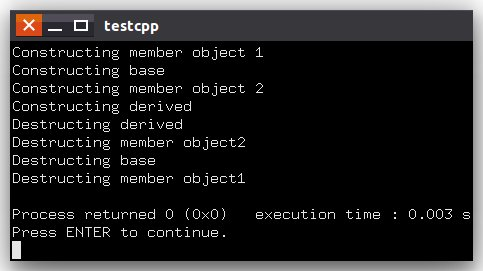
\includegraphics[width=0.6\textwidth]{figure/chap05/05ctorinit}};
    \end{tikzpicture}
  \end{center}
\end{frame}
  
%%%%%%%%%%%%%%%%%%%%%%%%%%%%%%%%%%%%%%%%%%%%%%%%%%%%%%%%%%%%%%%%%%%%%%%%%%%%%%%


\section[类型兼容]{类型兼容}\label{sec:chap05-sec04}
%%%%%%%%%%%%%%%%%%%%%%%%%%%%%% 类型兼容 %%%%%%%%%%%%%%%%%%%%%%%%%%%%%%%%%%
\begin{frame}[t, fragile]{类型兼容}{基本概念}%
  \stretchon
  \begin{itemize}
  \item \alert{类型兼容}:在公有派生的情况下,一个派生类对象可作为基类
    的对象来使用
    \begin{itemize}
    \item 派生类对象可以赋值给基类对象
    \item 派生类对象可以初始化基类的引用
    \item 派生类对象的地址可赋给指向基类的指针
    \end{itemize}
  \end{itemize}
  \stretchoff
\end{frame}

\begin{frame}[t, fragile]{类型兼容}{调用基本函数成员}%
  \begin{itemize}
  \item 如何通过派生类对象调用基类中被覆盖的成员函数
  \end{itemize}
  \begin{center}
    \begin{tikzpicture}[font=\tiny, show background grid]
      \tikzset{ coord/.style={coordinate} }
      
      \umlnote[text width=0.15\textwidth](code1) at (0, 0)
      {
        \begin{cppttnobg}
class CShape
{
public:
  ShowPos();
};
        \end{cppttnobg}
      };

      \umlnote[text width=0.35\textwidth,below=0.5 of code1](code2)
      {
        \begin{cppttnobg}
class CEllipse: public CShape
{
public:
  ShowPos();
};
        \end{cppttnobg}
      };

      \umlnote[text width=0.35\textwidth, right=of code2] (code3)
      {
        \begin{cppttnobg}
class CDonut: public CEllipse
{
public:
  ShowPos();
};
        \end{cppttnobg}
      };

      \umlnote[text width=0.35\textwidth, above=1 of code3] (note1)
      {
        \begin{cppttnobg}
CDonut myDonut;
myDonut.ShowPos();
        \end{cppttnobg}
      };

      \path let \p1=(note1) in
      coordinate (note10) at (\x1, \y1)
      coordinate (ovfun10) at ($(note10) + (-1.4, -0.35)$)
      coordinate (ovfun11) at ($(ovfun10) + (1.1, 0)$)
      coordinate (ovfunc1) at ($(ovfun10)!0.5!(ovfun11)$)
      ;

      \path let \p1=(code3) in
      coordinate (code30) at (\x1, \y1)
      coordinate (ovfun20) at ($(code30) + (-2.1, -0.5)$)
      coordinate (ovfun21) at ($(ovfun20) + (1.0, 0)$)
      coordinate (ovfunc2) at ($(ovfun20)!0.5!(ovfun21)$)
      ;

      \draw[red, thick] (ovfun10) -- (ovfun11);
      \draw[red, thick] (ovfun20) -- (ovfun21);

      \draw[-{Stealth[scale=1.0]}, blue, thick] (code1.south) to[out=-90,
      in=90] (code2.north);
      \draw[-{Stealth[scale=1.0]}, blue, thick] (code2.east) to[out=0,
      in=180] (code3.west);

      \draw[-{Stealth[scale=1.0]}, red, thick] (ovfun11.east) to[out=0,
      in=0] (ovfun21);
    \end{tikzpicture}
  \end{center}
\end{frame}

\begin{frame}[t, fragile]{类型兼容}{调用基本函数成员}%
  \begin{itemize}
  \item 如何通过派生类对象调用基类中被覆盖的成员函数
  \end{itemize}
  \begin{center}
    \begin{tikzpicture}[font=\tiny, show background grid]
      \tikzset{ coord/.style={coordinate} }
      
      \umlnote[text width=0.15\textwidth](code1) at (0, 0)
      {
        \begin{cppttnobg}
class CShape
{
public:
  ShowPos();
};
        \end{cppttnobg}
      };

      \umlnote[text width=0.35\textwidth,below=0.5 of code1](code2)
      {
        \begin{cppttnobg}
class CEllipse: public CShape
{
public:
  ShowPos();
};
        \end{cppttnobg}
      };

      \umlnote[text width=0.35\textwidth, right=of code2] (code3)
      {
        \begin{cppttnobg}
class CDonut: public CEllipse
{
public:
  ShowPos();
};
        \end{cppttnobg}
      };

      \umlnote[text width=0.35\textwidth, above=1 of code3] (note1)
      {
        \begin{cppttnobg}
CDonut myDonut;
myDonut.ShowPos();
        \end{cppttnobg}
      };

      \node[text width=0.35\textwidth] (question) at (6.2, -2)
      {
        \colorbox{green}{\textcolor{red}{\Large ?}}
      };

      \path let \p1=(note1) in
      coordinate (note10) at (\x1, \y1)
      coordinate (ovfun10) at ($(note10) + (-1.45, -0.4)$)
      coordinate (ovfun11) at ($(ovfun10) + (1.1, 0)$)
      coordinate (ovfunc1) at ($(ovfun10)!0.5!(ovfun11)$)
      ;

      \path let \p1=(code1) in
      coordinate (code10) at (\x1, \y1)
      coordinate (ovfun20) at ($(code10) + (-0.85, -0.45)$)
      coordinate (ovfun21) at ($(ovfun20) + (1.1, 0)$)
      coordinate (ovfunc2) at ($(ovfun20)!0.5!(ovfun21)$)
      ;

      \path let \p1=(code2) in
      coordinate (code20) at (\x1, \y1)
      coordinate (ovfun30) at ($(code20) + (-2.15, -0.52)$)
      coordinate (ovfun31) at ($(ovfun30) + (1.0, 0)$)
      coordinate (ovfunc3) at ($(ovfun30)!0.5!(ovfun31)$)
      ;

      \draw[red, thick] (ovfun10) -- (ovfun11);
      \draw[red, thick] (ovfun20) -- (ovfun21);
      \draw[red, thick] (ovfun30) -- (ovfun31);

      \draw[-{Stealth[scale=1.0]}, blue, thick] (code1.south) to[out=-90,
      in=90] (code2.north);
      \draw[-{Stealth[scale=1.0]}, blue, thick] (code2.east) to[out=0,
      in=180] (code3.west);

      \draw[-{Stealth[scale=1.0]}, red, thick] (ovfunc1) to[out=-90,
      in=-90] (ovfunc2);
      \draw[-{Stealth[scale=1.0]}, red, thick] (ovfunc1) to[out=-90,
      in=-90] (ovfunc3);
    \end{tikzpicture}
  \end{center}
\end{frame}

\begin{frame}[t, fragile]{类型兼容}{调用基本函数成员}%
  \begin{itemize}
  \item 如何通过派生类对象调用基类中被覆盖的成员函数
  \end{itemize}
  \begin{center}
    \begin{tikzpicture}[font=\tiny, show background grid]
      \tikzset{ coord/.style={coordinate} }
      
      \umlnote[text width=0.15\textwidth](code1) at (0, 0)
      {
        \begin{cppttnobg}
class CShape
{
public:
  ShowPos();
};
        \end{cppttnobg}
      };

      \umlnote[text width=0.35\textwidth,below=0.5 of code1](code2)
      {
        \begin{cppttnobg}
class CEllipse: public CShape
{
public:
  ShowPos();
};
        \end{cppttnobg}
      };

      \umlnote[text width=0.35\textwidth, right=of code2] (code3)
      {
        \begin{cppttnobg}
class CDonut: public CEllipse
{
public:
  ShowPos();
};
        \end{cppttnobg}
      };

      \umlnote[text width=0.35\textwidth, above=1 of code3] (note1)
      {
        \begin{cppttnobg}
CDonut myDonut;
CEllipse p = myDonut;
p.ShowPos();
        \end{cppttnobg}
      };      

      \path let \p1=(note1) in
      coordinate (note10) at (\x1, \y1)
      coordinate (ovfun10) at ($(note10) + (-2.15, -0.52)$)
      coordinate (ovfun11) at ($(ovfun10) + (1.3, 0)$)
      coordinate (ovfunc1) at ($(ovfun10)!0.5!(ovfun11)$)
      ;

      \path let \p1=(code1) in
      coordinate (code10) at (\x1, \y1)
      coordinate (ovfun20) at ($(code10) + (-0.85, -0.45)$)
      coordinate (ovfun21) at ($(ovfun20) + (1.1, 0)$)
      coordinate (ovfunc2) at ($(ovfun20)!0.5!(ovfun21)$)
      ;

      \path let \p1=(code2) in
      coordinate (code20) at (\x1, \y1)
      coordinate (ovfun30) at ($(code20) + (-2.15, -0.52)$)
      coordinate (ovfun31) at ($(ovfun30) + (1.0, 0)$)
      coordinate (ovfunc3) at ($(ovfun30)!0.5!(ovfun31)$)
      ;

      \draw[red, thick] (ovfun10) -- (ovfun11);
      %\draw[red, thick] (ovfun20) -- (ovfun21);
      \draw[red, thick] (ovfun30) -- (ovfun31);

      \draw[-{Stealth[scale=1.0]}, blue, thick] (code1.south) to[out=-90,
      in=90] (code2.north);
      \draw[-{Stealth[scale=1.0]}, blue, thick] (code2.east) to[out=0,
      in=180] (code3.west);

      % \draw[-{Stealth[scale=1.0]}, red, thick] (ovfunc1) to[out=-90,
      % in=-90] (ovfunc2);
      \draw[-{Stealth[scale=1.0]}, red, thick] (ovfunc1) to[out=-90,
      in=-90] (ovfunc3);
    \end{tikzpicture}
  \end{center}
\end{frame}

\begin{frame}[t, fragile]{类型兼容}{调用基本函数成员}%
  \begin{itemize}
  \item 如何通过派生类对象调用基类中被覆盖的成员函数
  \end{itemize}
  \begin{center}
    \begin{tikzpicture}[font=\tiny, show background grid]
      \tikzset{ coord/.style={coordinate} }
      
      \umlnote[text width=0.15\textwidth](code1) at (0, 0)
      {
        \begin{cppttnobg}
class CShape
{
public:
  ShowPos();
};
        \end{cppttnobg}
      };

      \umlnote[text width=0.35\textwidth,below=0.5 of code1](code2)
      {
        \begin{cppttnobg}
class CEllipse: public CShape
{
public:
  ShowPos();
};
        \end{cppttnobg}
      };

      \umlnote[text width=0.35\textwidth, right=of code2] (code3)
      {
        \begin{cppttnobg}
class CDonut: public CEllipse
{
public:
  ShowPos();
};
        \end{cppttnobg}
      };

      \umlnote[text width=0.35\textwidth, above=1 of code3] (note1)
      {
        \begin{cppttnobg}
CDonut myDonut;
CEllipse *p = &myDonut;
p->ShowPos();
        \end{cppttnobg}
      };      

      \path let \p1=(note1) in
      coordinate (note10) at (\x1, \y1)
      coordinate (ovfun10) at ($(note10) + (-2.15, -0.52)$)
      coordinate (ovfun11) at ($(ovfun10) + (1.3, 0)$)
      coordinate (ovfunc1) at ($(ovfun10)!0.5!(ovfun11)$)
      ;

      \path let \p1=(code1) in
      coordinate (code10) at (\x1, \y1)
      coordinate (ovfun20) at ($(code10) + (-0.85, -0.45)$)
      coordinate (ovfun21) at ($(ovfun20) + (1.1, 0)$)
      coordinate (ovfunc2) at ($(ovfun20)!0.5!(ovfun21)$)
      ;

      \path let \p1=(code2) in
      coordinate (code20) at (\x1, \y1)
      coordinate (ovfun30) at ($(code20) + (-2.15, -0.52)$)
      coordinate (ovfun31) at ($(ovfun30) + (1.1, 0)$)
      coordinate (ovfunc3) at ($(ovfun30)!0.5!(ovfun31)$)
      ;

      \draw[red, thick] (ovfun10) -- (ovfun11);
      %\draw[red, thick] (ovfun20) -- (ovfun21);
      \draw[red, thick] (ovfun30) -- (ovfun31);

      \draw[-{Stealth[scale=1.0]}, blue, thick] (code1.south) to[out=-90,
      in=90] (code2.north);
      \draw[-{Stealth[scale=1.0]}, blue, thick] (code2.east) to[out=0,
      in=180] (code3.west);

      % \draw[-{Stealth[scale=1.0]}, red, thick] (ovfunc1) to[out=-90,
      % in=-90] (ovfunc2);
      \draw[-{Stealth[scale=1.0]}, red, thick] (ovfunc1) to[out=-90,
      in=-90] (ovfunc3);
    \end{tikzpicture}
  \end{center}
\end{frame}

\begin{frame}[t, fragile]{类型兼容}{调用基本函数成员}%
  \begin{itemize}
  \item 如何通过派生类对象调用基类中被覆盖的成员函数
  \end{itemize}
  \begin{center}
    \begin{tikzpicture}[font=\tiny, show background grid]
      \tikzset{ coord/.style={coordinate} }
      
      \umlnote[text width=0.15\textwidth](code1) at (0, 0)
      {
        \begin{cppttnobg}
class CShape
{
public:
  ShowPos();
};
        \end{cppttnobg}
      };

      \umlnote[text width=0.35\textwidth,below=0.5 of code1](code2)
      {
        \begin{cppttnobg}
class CEllipse: public CShape
{
public:
  ShowPos();
};
        \end{cppttnobg}
      };

      \umlnote[text width=0.35\textwidth, right=of code2] (code3)
      {
        \begin{cppttnobg}
class CDonut: public CEllipse
{
public:
  ShowPos();
};
        \end{cppttnobg}
      };

      \umlnote[text width=0.35\textwidth, above=1 of code3] (note1)
      {
        \begin{cppttnobg}
CDonut myDonut;
CEllipse &p = myDonut;
p.ShowPos();
        \end{cppttnobg}
      };      

      \path let \p1=(note1) in
      coordinate (note10) at (\x1, \y1)
      coordinate (ovfun10) at ($(note10) + (-2.1, -0.52)$)
      coordinate (ovfun11) at ($(ovfun10) + (1.1, 0)$)
      coordinate (ovfunc1) at ($(ovfun10)!0.5!(ovfun11)$)
      ;

      \path let \p1=(code1) in
      coordinate (code10) at (\x1, \y1)
      coordinate (ovfun20) at ($(code10) + (-0.85, -0.45)$)
      coordinate (ovfun21) at ($(ovfun20) + (1.1, 0)$)
      coordinate (ovfunc2) at ($(ovfun20)!0.5!(ovfun21)$)
      ;

      \path let \p1=(code2) in
      coordinate (code20) at (\x1, \y1)
      coordinate (ovfun30) at ($(code20) + (-2.15, -0.52)$)
      coordinate (ovfun31) at ($(ovfun30) + (1.0, 0)$)
      coordinate (ovfunc3) at ($(ovfun30)!0.5!(ovfun31)$)
      ;

      \draw[red, thick] (ovfun10) -- (ovfun11);
      %\draw[red, thick] (ovfun20) -- (ovfun21);
      \draw[red, thick] (ovfun30) -- (ovfun31);

      \draw[-{Stealth[scale=1.0]}, blue, thick] (code1.south) to[out=-90,
      in=90] (code2.north);
      \draw[-{Stealth[scale=1.0]}, blue, thick] (code2.east) to[out=0,
      in=180] (code3.west);

      % \draw[-{Stealth[scale=1.0]}, red, thick] (ovfunc1) to[out=-90,
      % in=-90] (ovfunc2);
      \draw[-{Stealth[scale=1.0]}, red, thick] (ovfunc1) to[out=-90,
      in=-90] (ovfunc3);
    \end{tikzpicture}
  \end{center}
\end{frame}

\begin{frame}[t, fragile]{类型兼容}{调用基本函数成员}%
  \begin{itemize}
  \item 如何通过派生类对象调用基类中被覆盖的成员函数
  \end{itemize}
  \begin{center}
    \begin{tikzpicture}[font=\tiny, show background grid]
      \tikzset{ coord/.style={coordinate} }
      
      \umlnote[text width=0.15\textwidth](code1) at (0, 0)
      {
        \begin{cppttnobg}
class CShape
{
public:
  ShowPos();
};
        \end{cppttnobg}
      };

      \umlnote[text width=0.35\textwidth,below=0.5 of code1](code2)
      {
        \begin{cppttnobg}
class CEllipse: public CShape
{
public:
  ShowPos();
};
        \end{cppttnobg}
      };

      \umlnote[text width=0.35\textwidth, right=of code2] (code3)
      {
        \begin{cppttnobg}
class CDonut: public CEllipse
{
public:
  ShowPos();
};
        \end{cppttnobg}
      };

      \umlnote[text width=0.35\textwidth, above=1 of code3] (note1)
      {
        \begin{cppttnobg}
CDonut myDonut;
CShape p = myDonut;
p.ShowPos();
        \end{cppttnobg}
      };      

      \path let \p1=(note1) in
      coordinate (note10) at (\x1, \y1)
      coordinate (ovfun10) at ($(note10) + (-2.1, -0.52)$)
      coordinate (ovfun11) at ($(ovfun10) + (1.1, 0)$)
      coordinate (ovfunc1) at ($(ovfun10)!0.5!(ovfun11)$)
      ;

      \path let \p1=(code1) in
      coordinate (code10) at (\x1, \y1)
      coordinate (ovfun20) at ($(code10) + (-0.85, -0.45)$)
      coordinate (ovfun21) at ($(ovfun20) + (1.0, 0)$)
      coordinate (ovfunc2) at ($(ovfun20)!0.5!(ovfun21)$)
      ;

      \path let \p1=(code2) in
      coordinate (code20) at (\x1, \y1)
      coordinate (ovfun30) at ($(code20) + (-2.15, -0.52)$)
      coordinate (ovfun31) at ($(ovfun30) + (1.0, 0)$)
      coordinate (ovfunc3) at ($(ovfun30)!0.5!(ovfun31)$)
      ;

      \draw[red, thick] (ovfun10) -- (ovfun11);
      \draw[red, thick] (ovfun20) -- (ovfun21);
      %\draw[red, thick] (ovfun30) -- (ovfun31);

      \draw[-{Stealth[scale=1.0]}, blue, thick] (code1.south) to[out=-90,
      in=90] (code2.north);
      \draw[-{Stealth[scale=1.0]}, blue, thick] (code2.east) to[out=0,
      in=180] (code3.west);

      \draw[-{Stealth[scale=1.0]}, red, thick] (ovfunc1) to[out=-90,
      in=-90] (ovfunc2);
      % \draw[-{Stealth[scale=1.0]}, red, thick] (ovfunc1) to[out=-90,
      % in=-90] (ovfunc3);
    \end{tikzpicture}
  \end{center}
\end{frame}

\begin{frame}[t, fragile]{类型兼容}{调用基本函数成员}%
  \begin{itemize}
  \item 如何通过派生类对象调用基类中被覆盖的成员函数
  \end{itemize}
  \begin{center}
    \begin{tikzpicture}[font=\tiny, show background grid]
      \tikzset{ coord/.style={coordinate} }
      
      \umlnote[text width=0.15\textwidth](code1) at (0, 0)
      {
        \begin{cppttnobg}
class CShape
{
public:
  ShowPos();
};
        \end{cppttnobg}
      };

      \umlnote[text width=0.35\textwidth,below=0.5 of code1](code2)
      {
        \begin{cppttnobg}
class CEllipse: public CShape
{
public:
  ShowPos();
};
        \end{cppttnobg}
      };

      \umlnote[text width=0.35\textwidth, right=of code2] (code3)
      {
        \begin{cppttnobg}
class CDonut: public CEllipse
{
public:
  ShowPos();
};
        \end{cppttnobg}
      };

      \umlnote[text width=0.35\textwidth, above=1 of code3] (note1)
      {
        \begin{cppttnobg}
CDonut myDonut;
CShape *p = &myDonut;
p->ShowPos();
        \end{cppttnobg}
      };      

      \path let \p1=(note1) in
      coordinate (note10) at (\x1, \y1)
      coordinate (ovfun10) at ($(note10) + (-2.1, -0.52)$)
      coordinate (ovfun11) at ($(ovfun10) + (1.1, 0)$)
      coordinate (ovfunc1) at ($(ovfun10)!0.5!(ovfun11)$)
      ;

      \path let \p1=(code1) in
      coordinate (code10) at (\x1, \y1)
      coordinate (ovfun20) at ($(code10) + (-0.85, -0.45)$)
      coordinate (ovfun21) at ($(ovfun20) + (1.1, 0)$)
      coordinate (ovfunc2) at ($(ovfun20)!0.5!(ovfun21)$)
      ;

      \path let \p1=(code2) in
      coordinate (code20) at (\x1, \y1)
      coordinate (ovfun30) at ($(code20) + (-2.15, -0.52)$)
      coordinate (ovfun31) at ($(ovfun30) + (1.0, 0)$)
      coordinate (ovfunc3) at ($(ovfun30)!0.5!(ovfun31)$)
      ;

      \draw[red, thick] (ovfun10) -- (ovfun11);
      \draw[red, thick] (ovfun20) -- (ovfun21);
      %\draw[red, thick] (ovfun30) -- (ovfun31);

      \draw[-{Stealth[scale=1.0]}, blue, thick] (code1.south) to[out=-90,
      in=90] (code2.north);
      \draw[-{Stealth[scale=1.0]}, blue, thick] (code2.east) to[out=0,
      in=180] (code3.west);

      \draw[-{Stealth[scale=1.0]}, red, thick] (ovfunc1) to[out=-90,
      in=-90] (ovfunc2);
      % \draw[-{Stealth[scale=1.0]}, red, thick] (ovfunc1) to[out=-90,
      % in=-90] (ovfunc3);
    \end{tikzpicture}
  \end{center}
\end{frame}

\begin{frame}[t, fragile]{类型兼容}{调用基本函数成员}%
  \begin{itemize}
  \item 如何通过派生类对象调用基类中被覆盖的成员函数
  \end{itemize}
  \begin{center}
    \begin{tikzpicture}[font=\tiny, show background grid]
      \tikzset{ coord/.style={coordinate} }
      
      \umlnote[text width=0.15\textwidth](code1) at (0, 0)
      {
        \begin{cppttnobg}
class CShape
{
public:
  ShowPos();
};
        \end{cppttnobg}
      };

      \umlnote[text width=0.35\textwidth,below=0.5 of code1](code2)
      {
        \begin{cppttnobg}
class CEllipse: public CShape
{
public:
  ShowPos();
};
        \end{cppttnobg}
      };

      \umlnote[text width=0.35\textwidth, right=of code2] (code3)
      {
        \begin{cppttnobg}
class CDonut: public CEllipse
{
public:
  ShowPos();
};
        \end{cppttnobg}
      };

      \umlnote[text width=0.35\textwidth, above=1 of code3] (note1)
      {
        \begin{cppttnobg}
CDonut myDonut;
CShape &p = myDonut;
p.ShowPos();
        \end{cppttnobg}
      };      

      \path let \p1=(note1) in
      coordinate (note10) at (\x1, \y1)
      coordinate (ovfun10) at ($(note10) + (-2.1, -0.52)$)
      coordinate (ovfun11) at ($(ovfun10) + (1.1, 0)$)
      coordinate (ovfunc1) at ($(ovfun10)!0.5!(ovfun11)$)
      ;

      \path let \p1=(code1) in
      coordinate (code10) at (\x1, \y1)
      coordinate (ovfun20) at ($(code10) + (-0.85, -0.45)$)
      coordinate (ovfun21) at ($(ovfun20) + (1.0, 0)$)
      coordinate (ovfunc2) at ($(ovfun20)!0.5!(ovfun21)$)
      ;

      \path let \p1=(code2) in
      coordinate (code20) at (\x1, \y1)
      coordinate (ovfun30) at ($(code20) + (-2.15, -0.52)$)
      coordinate (ovfun31) at ($(ovfun30) + (1.0, 0)$)
      coordinate (ovfunc3) at ($(ovfun30)!0.5!(ovfun31)$)
      ;

      \draw[red, thick] (ovfun10) -- (ovfun11);
      \draw[red, thick] (ovfun20) -- (ovfun21);
      %\draw[red, thick] (ovfun30) -- (ovfun31);

      \draw[-{Stealth[scale=1.0]}, blue, thick] (code1.south) to[out=-90,
      in=90] (code2.north);
      \draw[-{Stealth[scale=1.0]}, blue, thick] (code2.east) to[out=0,
      in=180] (code3.west);

      \draw[-{Stealth[scale=1.0]}, red, thick] (ovfunc1) to[out=-90,
      in=-90] (ovfunc2);
      % \draw[-{Stealth[scale=1.0]}, red, thick] (ovfunc1) to[out=-90,
      % in=-90] (ovfunc3);
    \end{tikzpicture}
  \end{center}
\end{frame}

\begin{frame}[t, fragile]{类型兼容}{调用基本函数成员}%
  \begin{itemize}
  \item 如何通过派生类对象调用基类中被覆盖的成员函数
  \end{itemize}
  \begin{center}
    \begin{tikzpicture}[font=\tiny, show background grid]
      \tikzset{ coord/.style={coordinate} }
      
      \umlnote[text width=0.15\textwidth](code1) at (0, 0)
      {
        \begin{cppttnobg}
class CShape
{
public:
  ShowPos();
};
        \end{cppttnobg}
      };

      \umlnote[text width=0.35\textwidth,below=0.5 of code1](code2)
      {
        \begin{cppttnobg}
class CEllipse: public CShape
{
public:
  ShowPos();
};
        \end{cppttnobg}
      };

      \umlnote[text width=0.35\textwidth, right=of code2] (code3)
      {
        \begin{cppttnobg}
class CDonut: public CEllipse
{
public:
  ShowPos();
};
        \end{cppttnobg}
      };

      \umlnote[text width=0.2\textwidth, xshift=-1.8cm, above=1 of code3] (note1)
      {
        \begin{cppttnobg}
CDonut myDonut;
Show(myDonut);
        \end{cppttnobg}
      };

      \umlnote[text width=0.25\textwidth, right=0.5 of note1] (note2)
      {
        \begin{cppttnobg}
void Show(CShape p)
{
  p.ShowPos();
}
        \end{cppttnobg}
      }; 

      \path let \p1=(note1) in
      coordinate (note10) at (\x1, \y1)
      coordinate (ovfun10) at ($(note10) + (-1.3, -0.4)$)
      coordinate (ovfun11) at ($(ovfun10) + (1.3, 0)$)
      coordinate (ovfunc1) at ($(ovfun10)!0.5!(ovfun11)$)
      ;

      \path let \p1=(code1) in
      coordinate (code10) at (\x1, \y1)
      coordinate (ovfun20) at ($(code10) + (-0.85, -0.45)$)
      coordinate (ovfun21) at ($(ovfun20) + (1.0, 0)$)
      coordinate (ovfunc2) at ($(ovfun20)!0.5!(ovfun21)$)
      ;

      \path let \p1=(code2) in
      coordinate (code20) at (\x1, \y1)
      coordinate (ovfun30) at ($(code20) + (-1.6, -0.55)$)
      coordinate (ovfun31) at ($(ovfun30) + (1.1, 0)$)
      coordinate (ovfunc3) at ($(ovfun30)!0.5!(ovfun31)$)
      ;

      \draw[red, thick] (ovfun10) -- (ovfun11);
      \draw[red, thick] (ovfun20) -- (ovfun21);
      %\draw[red, thick] (ovfun30) -- (ovfun31);

      \draw[-{Stealth[scale=1.0]}, blue, thick] (code1.south) to[out=-90,
      in=90] (code2.north);
      \draw[-{Stealth[scale=1.0]}, blue, thick] (code2.east) to[out=0,
      in=180] (code3.west);

      \draw[-{Stealth[scale=1.0]}, red, thick] (ovfunc1) to[out=-90,
      in=-90] (ovfunc2);
      % \draw[-{Stealth[scale=1.0]}, red, thick] (ovfunc1) to[out=-90,
      % in=-90] (ovfunc3);
    \end{tikzpicture}
  \end{center}
\end{frame}

\begin{frame}[t, fragile]{类型兼容}{调用基本函数成员}%
  \begin{itemize}
  \item 如何通过派生类对象调用基类中被覆盖的成员函数
  \end{itemize}
  \begin{center}
    \begin{tikzpicture}[font=\tiny, show background grid]
      \tikzset{ coord/.style={coordinate} }
      
      \umlnote[text width=0.15\textwidth](code1) at (0, 0)
      {
        \begin{cppttnobg}
class CShape
{
public:
  ShowPos();
};
        \end{cppttnobg}
      };

      \umlnote[text width=0.35\textwidth,below=0.5 of code1](code2)
      {
        \begin{cppttnobg}
class CEllipse: public CShape
{
public:
  ShowPos();
};
        \end{cppttnobg}
      };

      \umlnote[text width=0.35\textwidth, right=of code2] (code3)
      {
        \begin{cppttnobg}
class CDonut: public CEllipse
{
public:
  ShowPos();
};
        \end{cppttnobg}
      };

      \umlnote[text width=0.2\textwidth, xshift=-1.8cm, above=1 of code3] (note1)
      {
        \begin{cppttnobg}
CDonut myDonut;
Show(&myDonut);
        \end{cppttnobg}
      };

      \umlnote[text width=0.25\textwidth, right=0.5 of note1] (note2)
      {
        \begin{cppttnobg}
void Show(CShape *p)
{
  p->ShowPos();
}
        \end{cppttnobg}
      }; 

      \path let \p1=(note1) in
      coordinate (note10) at (\x1, \y1)
      coordinate (ovfun10) at ($(note10) + (-1.3, -0.4)$)
      coordinate (ovfun11) at ($(ovfun10) + (1.4, 0)$)
      coordinate (ovfunc1) at ($(ovfun10)!0.5!(ovfun11)$)
      ;

      \path let \p1=(code1) in
      coordinate (code10) at (\x1, \y1)
      coordinate (ovfun20) at ($(code10) + (-0.85, -0.45)$)
      coordinate (ovfun21) at ($(ovfun20) + (1.0, 0)$)
      coordinate (ovfunc2) at ($(ovfun20)!0.5!(ovfun21)$)
      ;

      \path let \p1=(code2) in
      coordinate (code20) at (\x1, \y1)
      coordinate (ovfun30) at ($(code20) + (-2.15, -0.52)$)
      coordinate (ovfun31) at ($(ovfun30) + (1.0, 0)$)
      coordinate (ovfunc3) at ($(ovfun30)!0.5!(ovfun31)$)
      ;

      \draw[red, thick] (ovfun10) -- (ovfun11);
      \draw[red, thick] (ovfun20) -- (ovfun21);
      %\draw[red, thick] (ovfun30) -- (ovfun31);

      \draw[-{Stealth[scale=1.0]}, blue, thick] (code1.south) to[out=-90,
      in=90] (code2.north);
      \draw[-{Stealth[scale=1.0]}, blue, thick] (code2.east) to[out=0,
      in=180] (code3.west);

      \draw[-{Stealth[scale=1.0]}, red, thick] (ovfunc1) to[out=-90,
      in=-90] (ovfunc2);
      % \draw[-{Stealth[scale=1.0]}, red, thick] (ovfunc1) to[out=-90,
      % in=-90] (ovfunc3);
    \end{tikzpicture}
  \end{center}
\end{frame}

\begin{frame}[t, fragile]{类型兼容}{调用基本函数成员}%
  \begin{itemize}
  \item 如何通过派生类对象调用基类中被覆盖的成员函数
  \end{itemize}
  \begin{center}
    \begin{tikzpicture}[font=\tiny, show background grid]
      \tikzset{ coord/.style={coordinate} }
      
      \umlnote[text width=0.15\textwidth](code1) at (0, 0)
      {
        \begin{cppttnobg}
class CShape
{
public:
  ShowPos();
};
        \end{cppttnobg}
      };

      \umlnote[text width=0.35\textwidth,below=0.5 of code1](code2)
      {
        \begin{cppttnobg}
class CEllipse: public CShape
{
public:
  ShowPos();
};
        \end{cppttnobg}
      };

      \umlnote[text width=0.35\textwidth, right=of code2] (code3)
      {
        \begin{cppttnobg}
class CDonut: public CEllipse
{
public:
  ShowPos();
};
        \end{cppttnobg}
      };

      \umlnote[text width=0.2\textwidth, xshift=-1.8cm, above=1 of code3] (note1)
      {
        \begin{cppttnobg}
CDonut myDonut;
Show(myDonut);
        \end{cppttnobg}
      };

      \umlnote[text width=0.25\textwidth, right=0.5 of note1] (note2)
      {
        \begin{cppttnobg}
void Show(CShape &p)
{
  p.ShowPos();
}
        \end{cppttnobg}
      }; 

      \path let \p1=(note1) in
      coordinate (note10) at (\x1, \y1)
      coordinate (ovfun10) at ($(note10) + (-1.3, -0.4)$)
      coordinate (ovfun11) at ($(ovfun10) + (1.4, 0)$)
      coordinate (ovfunc1) at ($(ovfun10)!0.5!(ovfun11)$)
      ;

      \path let \p1=(code1) in
      coordinate (code10) at (\x1, \y1)
      coordinate (ovfun20) at ($(code10) + (-0.85, -0.45)$)
      coordinate (ovfun21) at ($(ovfun20) + (1.05, 0)$)
      coordinate (ovfunc2) at ($(ovfun20)!0.5!(ovfun21)$)
      ;

      \path let \p1=(code2) in
      coordinate (code20) at (\x1, \y1)
      coordinate (ovfun30) at ($(code20) + (-2.15, -0.52)$)
      coordinate (ovfun31) at ($(ovfun30) + (1.05, 0)$)
      coordinate (ovfunc3) at ($(ovfun30)!0.5!(ovfun31)$)
      ;

      \draw[red, thick] (ovfun10) -- (ovfun11);
      \draw[red, thick] (ovfun20) -- (ovfun21);
      %\draw[red, thick] (ovfun30) -- (ovfun31);

      \draw[-{Stealth[scale=1.0]}, blue, thick] (code1.south) to[out=-90,
      in=90] (code2.north);
      \draw[-{Stealth[scale=1.0]}, blue, thick] (code2.east) to[out=0,
      in=180] (code3.west);

      \draw[-{Stealth[scale=1.0]}, red, thick] (ovfunc1) to[out=-90,
      in=-90] (ovfunc2);
      % \draw[-{Stealth[scale=1.0]}, red, thick] (ovfunc1) to[out=-90,
      % in=-90] (ovfunc3);
    \end{tikzpicture}
  \end{center}
\end{frame}
%%%%%%%%%%%%%%%%%%%%%%%%%%%%%%%%%%%%%%%%%%%%%%%%%%%%%%%%%%%%%%%%%%%%%%%%%%%%%%%

\section[多继承]{多继承}\label{sec:chap05-sec05}
%%%%%%%%%%%%%%%%%%%%%%%%%%%%%% 多继承 %%%%%%%%%%%%%%%%%%%%%%%%%%%%%%%%%%
\begin{frame}[t, fragile]{多继承}{基本概念}%
  \begin{itemize}
  \item 飞马(Pegasus)
  \end{itemize}
  \begin{center}
     \begin{tikzpicture}[font=\tiny, show background grid]
      \tikzset{ coord/.style={coordinate} }

      \begin{class}[fill=green!25, text width=3em]{马horse}{0 ,0}
      \end{class}
      
      \begin{class}[fill=green!25, text width=3em]{鸟bird}{5 ,0}
      \end{class}

      \begin{class}[fill=blue!25, text width=5em]{飞马pegasus}{2.5, -2.5}
        \inherit{马horse}
        \inherit{鸟bird}
      \end{class}

      \node[inner sep=0pt, above=0.1 of 马horse] (horse)
      {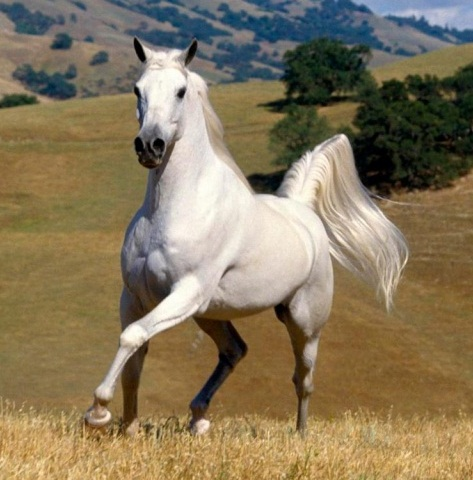
\includegraphics[width=.15\textwidth]{chap05/06-01horse}};
           
      \node[inner sep=0pt, above=0.1 of 鸟bird] (bird)
      {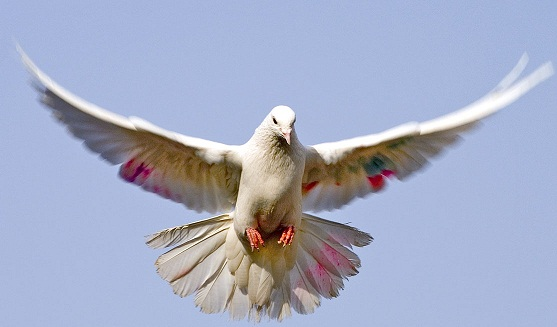
\includegraphics[width=.15\textwidth]{chap05/06-02bird}};
      
      \node[inner sep=0pt, above=0.13 of 飞马pegasus] (horsebird) 
      {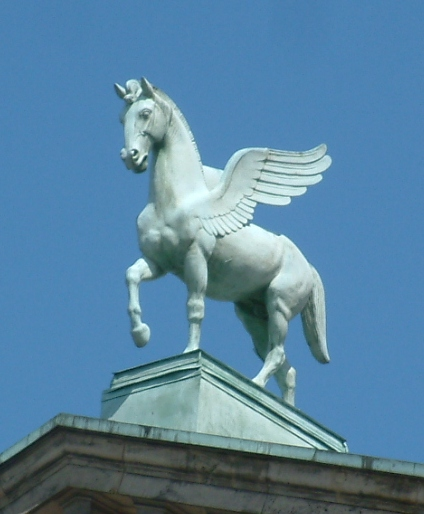
\includegraphics[width=.12\textwidth]{chap05/06-03horsebird}};      
    \end{tikzpicture}    
  \end{center}
\end{frame}

\begin{frame}[t, fragile]{多继承}{基本概念}%
  \begin{itemize}
  \item 飞马(Pegasus)
  \end{itemize}
  \begin{center}
     \begin{tikzpicture}[font=\tiny, show background grid]
      \tikzset{ coord/.style={coordinate} }

      \begin{class}[fill=red!25, text width=3em]{动物类CAnimal}{0, 0}
      \end{class}

      \begin{class}[fill=green!25, text width=3em]{马CHorse}{-3, -2}
        \inherit{动物类CAnimal}
      \end{class}
      
      \begin{class}[fill=green!25, text width=3em]{鸟CBird}{3, -2}
        \inherit{动物类CAnimal}
      \end{class}

      \begin{class}[fill=blue!25, text width=5em]{飞马CPegasus}{0, -4}
        \inherit{马CHorse}
        \inherit{鸟CBird}
      \end{class}   
    \end{tikzpicture}    
  \end{center}
\end{frame}

\begin{frame}[t, fragile]{多继承}{基本概念}%
  \begin{itemize}
  \item 代码示例
  \end{itemize}
  \begin{center}
    \begin{tikzpicture}[font=\tiny, show background grid]
      \tikzset{ coord/.style={coordinate} }
      
      \umlnote[scale = 0.9, text width=0.3\textwidth](note1) at (0, 0)
      {
        \cppfilettnobg{codes/chap05/05-09basecls.cpp}
      };

      \umlnote[scale = 0.9, text width=0.45\textwidth](note2) at (5, 0)
      {
        \cppfilettnobg{codes/chap05/05-09inheritcls.cpp}
      };

      \umlnote[scale = 0.9, text width=0.45\textwidth](note2) at (5, -4)
      {
        \cppfilettnobg{codes/chap05/05-09maincls.cpp}
      };
    \end{tikzpicture}
  \end{center}
\end{frame}

\begin{frame}[t, fragile]{多继承}{构造与析构}%
  \stretchon
  \begin{itemize}
  \item 多继承的构造与析构
    \begin{itemize}
    \item 调用各基类构造函数:调用顺序按基类被继承时声明的顺序,从左向
      右依次进行
    \item 调用派生类成员对象构造函数:调用顺序按其在类中定义的顺序依次
      执行
    \item 调用派生类构造函数
    \end{itemize}
  \end{itemize}
  \stretchoff
\end{frame}

\begin{frame}[t, fragile]{多继承}{构造与析构}%
  \begin{itemize}
  \item 代码示例
  \end{itemize}
  \begin{center}
    \begin{tikzpicture}[font=\tiny, show background grid]
      \tikzset{ coord/.style={coordinate} }
      
      \umlnote[scale = 0.9, text width=0.4\textwidth](note1) at (0, 0)
      {
        \cppfilettnobg{codes/chap05/05-10multibase.cpp}
      };

      \umlnote[scale = 0.9, text width=0.45\textwidth](note2) at (5, 0)
      {
        \cppfilettnobg{codes/chap05/05-10multibasectormain.cpp}
      };

       \node[inner sep=0pt, below=0.2 of note2] (ctor) 
      {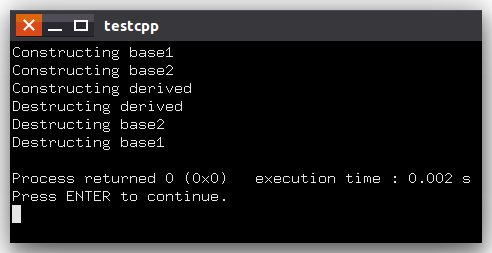
\includegraphics[width=.3\textwidth]{chap05/07-multiInheritCtor}};  
     
    \end{tikzpicture}
  \end{center}
\end{frame}

\begin{frame}[t, fragile]{多继承}{飞马类设计}%
  \begin{itemize}
  \item 飞马(Pegasus)
  \end{itemize}
  \begin{center}
     \begin{tikzpicture}[font=\tiny, show background grid]
      \tikzset{ coord/.style={coordinate} }

      \begin{class}[fill=green!25, text width=3em]{马horse}{0 ,0}
      \end{class}
      
      \begin{class}[fill=green!25, text width=3em]{鸟bird}{5 ,0}
      \end{class}

      \begin{class}[fill=blue!25, text width=5em]{飞马pegasus}{2.5, -2.5}
        \inherit{马horse}
        \inherit{鸟bird}
      \end{class}

      \node[inner sep=0pt, above=0.1 of 马horse] (horse)
      {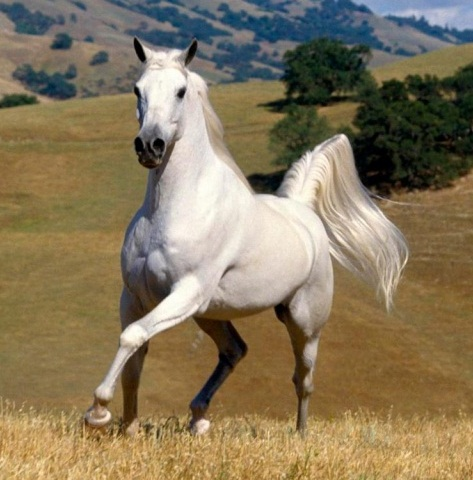
\includegraphics[width=.15\textwidth]{chap05/06-01horse}};
           
      \node[inner sep=0pt, above=0.1 of 鸟bird] (bird)
      {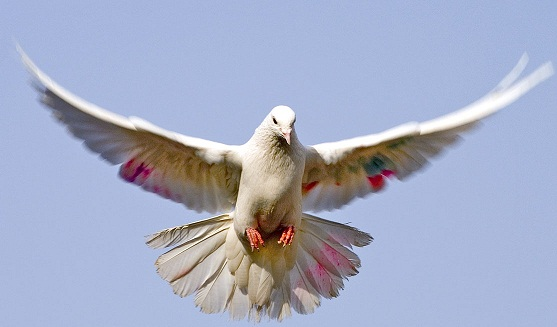
\includegraphics[width=.15\textwidth]{chap05/06-02bird}};
      
      \node[inner sep=0pt, above=0.13 of 飞马pegasus] (horsebird) 
      {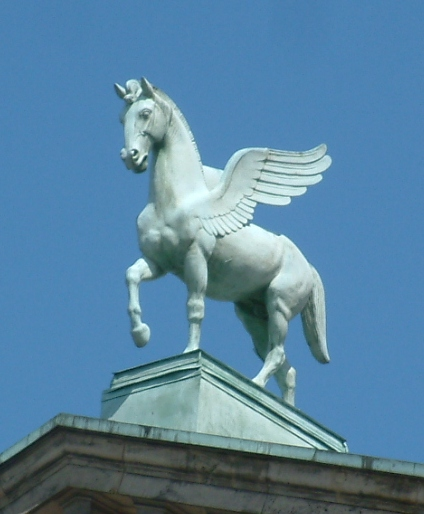
\includegraphics[width=.12\textwidth]{chap05/06-03horsebird}};      
    \end{tikzpicture}    
  \end{center}
\end{frame}

\begin{frame}[t, fragile]{多继承}{飞马类设计}%
  \begin{itemize}
  \item 飞马(Pegasus)
  \end{itemize}
  \begin{center}
     \begin{tikzpicture}[font=\tiny, show background grid]
      \tikzset{ coord/.style={coordinate} }

      \begin{class}[fill=red!25, text width=3em]{动物类CAnimal}{0, 0}
      \end{class}

      \begin{class}[fill=green!25, text width=3em]{马CHorse}{-3, -2}
        \inherit{动物类CAnimal}
      \end{class}
      
      \begin{class}[fill=green!25, text width=3em]{鸟CBird}{3, -2}
        \inherit{动物类CAnimal}
      \end{class}

      \begin{class}[fill=blue!25, text width=5em]{飞马CPegasus}{0, -4}
        \inherit{马CHorse}
        \inherit{鸟CBird}
      \end{class}   
    \end{tikzpicture}    
  \end{center}
\end{frame}

\begin{frame}[t, fragile]{多继承}{飞马类设计}%
  \begin{itemize}
  \item 飞马(Pegasus)
  \end{itemize}
  \begin{center}
     \begin{tikzpicture}[font=\tiny, show background grid]
      \tikzset{ coord/.style={coordinate} }

      \begin{class}[fill=red!25, text width=4em]{动物类CAnimal}{0, 0}
        \attribute{-name[32]:char}
        \attribute{-age:int}
        \attribute{-weight:int}
        \operation{+show():void}
      \end{class}

      \begin{class}[fill=green!25, text width=4em]{马CHorse}{-3, -2}
        \inherit{动物类CAnimal}
        \attribute{-power:int}
        \operation{+show():void}
        \operation{+talk():void}
        \operation{+run():void}
      \end{class}
      
      \begin{class}[fill=green!25, text width=4em]{鸟CBird}{3, -2}
        \inherit{动物类CAnimal}
        \attribute{-wingSpan:int}
        \operation{+show():void}
        \operation{+talk():void}
        \operation{+fly():void}
      \end{class}

      \begin{class}[fill=blue!25, text width=4em]{飞马CPegasus}{0, -4}
        \inherit{马CHorse}
        \inherit{鸟CBird}
        \operation{+show():void}
      \end{class}

      \path let \p1=(马CHorse) in
      coordinate (note10) at (\x1, \y1)
      coordinate (ovBL1) at ($(note10) + (-0.85, -0.35)$)
      coordinate (ovUR1) at ($(ovBL1) + (1.45, 0.3)$)
      coordinate (ovCD1) at ($(ovBL1)!0.5!(ovUR1)$)
      coordinate (ovCR1) at (ovUR1|-ovCD1)
      ;

     \path let \p1=(鸟CBird) in
      coordinate (note10) at (\x1, \y1)
      coordinate (ovBL2) at ($(note10) + (-0.85, -0.35)$)
      coordinate (ovUR2) at ($(ovBL2) + (1.45, 0.3)$)
      coordinate (ovCD2) at ($(ovBL2)!0.5!(ovUR2)$)
      coordinate (ovCR2) at (ovUR2|-ovCD2)
      ;
      
      \draw[red,thick,fill=green!25, fill opacity=0.14](ovBL1) rectangle
      (ovUR1);
      \draw[red,thick,fill=green!25, fill opacity=0.14](ovBL2) rectangle
      (ovUR2);      
    \end{tikzpicture}    
  \end{center}
\end{frame}

\begin{frame}[t, fragile]{多继承}{飞马类实例代码}%
  \begin{itemize}
  \item 动物类
  \end{itemize}
  %\vspace{-2ex}
  \begin{center}
    \begin{tikzpicture}[font=\tiny, show background grid]
      \tikzset{ coord/.style={coordinate} }
      
      \umlnote[scale = 0.9, text width=0.65\textwidth](note1) at (0, 0)
      {
        \cppfilettnobg{codes/chap05/05-11CAnimal.cpp}
      };
    \end{tikzpicture}
  \end{center}
\end{frame}

\begin{frame}[t, fragile]{多继承}{飞马类实例代码}%
  \begin{itemize}
  \item 鸟类
  \end{itemize}
  %\vspace{-2ex}
  \begin{center}
    \begin{tikzpicture}[font=\tiny, show background grid]
      \tikzset{ coord/.style={coordinate} }
      
      \umlnote[scale = 0.9, text width=0.85\textwidth](note1) at (0, 0)
      {
        \cppfilettnobg{codes/chap05/05-11CBird.cpp}
      };
    \end{tikzpicture}
  \end{center}
\end{frame}

\begin{frame}[t, fragile]{多继承}{飞马类实例代码}%
  \begin{itemize}
  \item 马类
  \end{itemize}
  %\vspace{-2ex}
  \begin{center}
    \begin{tikzpicture}[font=\tiny, show background grid]
      \tikzset{ coord/.style={coordinate} }
      
      \umlnote[scale = 0.9, text width=0.85\textwidth](note2) at (5, 0)
      {
        \cppfilettnobg{codes/chap05/05-11CHorse.cpp}
      };

    \end{tikzpicture}
  \end{center}
\end{frame}

\begin{frame}[t, fragile]{多继承}{飞马类实例代码}%
  \begin{itemize}
  \item 飞马类
  \end{itemize}
  \begin{center}
    \begin{tikzpicture}[font=\tiny, show background grid]
      \tikzset{ coord/.style={coordinate} }
      
      \umlnote[scale = 0.9, text width=0.85\textwidth](note1) at (0, 0)
      {
        \cppfilettnobg{codes/chap05/05-11CPegasus.cpp}
      };
    \end{tikzpicture}
  \end{center}
\end{frame}

\begin{frame}[t, fragile]{多继承}{二义性问题}%
  \begin{itemize}
  \item 多继承的二义性问题
  \end{itemize}
  \begin{center}
     \begin{tikzpicture}[font=\tiny, show background grid]
      \tikzset{ coord/.style={coordinate} }

      \begin{class}[fill=red!25, text width=4em]{动物类CAnimal}{0, 0}
        \attribute{-name[32]:char}
        \attribute{-age:int}
        \attribute{-weight:int}
        \operation{+show():void}
      \end{class}

      \begin{class}[fill=green!25, text width=4em]{马CHorse}{-3, -2}
        \inherit{动物类CAnimal}
        \attribute{-power:int}
        \operation{+show():void}
        \operation{+talk():void}
        \operation{+run():void}
      \end{class}
      
      \begin{class}[fill=green!25, text width=4em]{鸟CBird}{3, -2}
        \inherit{动物类CAnimal}
        \attribute{-wingSpan:int}
        \operation{+show():void}
        \operation{+talk():void}
        \operation{+fly():void}
      \end{class}

      \begin{class}[fill=blue!25, text width=4em]{飞马CPegasus}{0, -4}
        \inherit{马CHorse}
        \inherit{鸟CBird}
        \operation{+talk():void}
      \end{class}

      \path let \p1=(马CHorse) in
      coordinate (note10) at (\x1, \y1)
      coordinate (ovBL1) at ($(note10) + (-0.85, -0.35)$)
      coordinate (ovUR1) at ($(ovBL1) + (1.45, 0.3)$)
      coordinate (ovCD1) at ($(ovBL1)!0.5!(ovUR1)$)
      coordinate (ovCR1) at (ovUR1|-ovCD1)
      ;

     \path let \p1=(鸟CBird) in
      coordinate (note10) at (\x1, \y1)
      coordinate (ovBL2) at ($(note10) + (-0.85, -0.35)$)
      coordinate (ovUR2) at ($(ovBL2) + (1.45, 0.3)$)
      coordinate (ovCD2) at ($(ovBL2)!0.5!(ovUR2)$)
      coordinate (ovCR2) at (ovUR2|-ovCD2)
      ;
      
      \draw[red,thick,fill=green!25, fill opacity=0.14](ovBL1) rectangle
      (ovUR1);
      \draw[red,thick,fill=green!25, fill opacity=0.14](ovBL2) rectangle
      (ovUR2);      
    \end{tikzpicture}    
  \end{center}
\end{frame}

\begin{frame}[t, fragile]{多继承}{二义性问题}%
  \begin{itemize}
  \item 派生类的多个基类中拥有同名成员时,继承后通过对象调用同名成员将出现二义性
  \end{itemize}
  \begin{center}
    \begin{tikzpicture}[font=\tiny, show background grid]
      \tikzset{ coord/.style={coordinate} }
      
      \umlnote[text width=0.5\textwidth](code1) at (0, 0)
      {
        \begin{cppttnobg}
CPegasus pegObj("Pegasus", 5, 800, 2, 10000);
|\textcolor{red}{pegObj.Show(); \large \badmark}|
        \end{cppttnobg}
      };
      
      \node[anchor=north west, below=0.5 of code1] (fig) {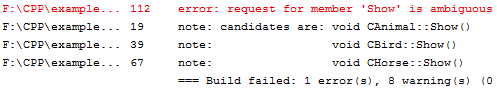
\includegraphics[width=0.8\textwidth]{figure/chap05/08-ambiguous}};
    \end{tikzpicture}
  \end{center}
\end{frame}

\begin{frame}[t, fragile]{多继承}{二义性问题}%
  \begin{spacing}{1.8}
  \begin{itemize}
  \item 解决方法1:类型兼容
  \end{itemize}
  \begin{center}
    \begin{tikzpicture}[font=\tiny, show background grid]
      \tikzset{ coord/.style={coordinate} }
      
      \umlnote[text width=0.5\textwidth](code1) at (0, 0)
      {
        \begin{cppttnobg}
CPegasus pegObj("Pegasus", 5, 800, 2, 10000);
CBird birdObj = pegObj;
birdObj.Show();
CHorse horObj = pegObj;
horObj.Show();
        \end{cppttnobg}
      };
    \end{tikzpicture}
  \end{center}
  \end{spacing}
\end{frame}

\begin{frame}[t, fragile]{多继承}{二义性问题}%
  \begin{spacing}{1.6}
  \begin{itemize}
  \item 解决方法2:成员重定义
  \end{itemize}
  \begin{center}
    \begin{tikzpicture}[font=\tiny, show background grid]
      \tikzset{ coord/.style={coordinate} }

      \begin{class}[fill=blue!25, text width=4em]{飞马CPegasus}{0, 0}        
        \operation{+talk():void}
        \operation{+Show():void}
      \end{class}

      \umlnote[text width=0.2\textwidth, below=0.2 of 飞马CPegasus](code1) 
      {
        \begin{cppttnobg}
void Show()
{
   CBird::Show();
   CHorse::Show();
}
        \end{cppttnobg}
      };
      
      \umlnote[text width=0.5\textwidth, below=0.2 of code1](code2) 
      {
        \begin{cppttnobg}
CPegasus pegObj("Pegasus", 5, 800, 2, 10000);
pegObj.Show();
        \end{cppttnobg}
      };
    \end{tikzpicture}
  \end{center}
  \end{spacing}
\end{frame}

\begin{frame}[t, fragile]{多继承}{二义性问题}%
  \begin{itemize}
  \item 间接二义性:基类构造函数两次被调用
  \end{itemize}
  \begin{center}
    \begin{tikzpicture}[font=\tiny, show background grid]
      \tikzset{ coord/.style={coordinate} }

      \umlnote[scale=0.95,text width=0.75\textwidth](code1) at (0, 0)
      {
        \begin{cppttnobg}
CPegasus(char *strName="", int a=0, int w=0, int ws=0,intpow=0):
                 CHorse(pow, strName, a,w), CBird(ws, strName, a, w) 
{
     cout << "Pegasus constructor" << endl;
}
|\vdots|
int main()
{
    CPegasus pegObj("Pegasus", 5, 100, 2, 500);
    return 0;
}
        \end{cppttnobg}
      };

      \node[anchor=north west, below=0.1 of code1] (fig)
      {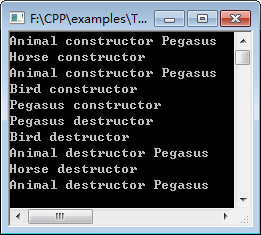
\includegraphics[width=0.25\textwidth]{figure/chap05/09-ctor-ambiguous}};
      \path let \p1=(fig) in
      coordinate (org) at (\x1, \y1)
      coordinate (ovBL1) at ($(org) + (-1.55, 0.83)$)
      coordinate (ovUR1) at ($(ovBL1) + (2.67, 0.22)$)
      coordinate (ovBL2) at ($(org) + (-1.55, 0.43)$)
      coordinate (ovUR2) at ($(ovBL2) + (2.67, 0.22)$)
      ;

      \draw[red,thick,fill=green!25, fill opacity=0.14](ovBL1) rectangle
      (ovUR1);
      \draw[red,thick,fill=green!25, fill opacity=0.14](ovBL2) rectangle
      (ovUR2); 
      
    \end{tikzpicture}
  \end{center}
\end{frame}

\begin{frame}[t, fragile]{多继承}{二义性问题}%
  \begin{itemize}
  \item 同名数据成员在内存中同时拥有多个拷贝
  \end{itemize}
  \begin{center}
     \begin{tikzpicture}[font=\tiny, show background grid]
      \tikzset{ coord/.style={coordinate} }

      \begin{class}[fill=red!25, text width=4em]{动物类CAnimal}{0, 0}
        \attribute{-name[32]:char}
        \attribute{-age:int}
        \attribute{-weight:int}
        \operation{+show():void}
      \end{class}

      \begin{class}[fill=green!25, text width=4em]{马CHorse}{-3, -2}
        \inherit{动物类CAnimal}
        \attribute{-power:int}
        \operation{+show():void}
        \operation{+talk():void}
        \operation{+run():void}
      \end{class}
      
      \begin{class}[fill=green!25, text width=4em]{鸟CBird}{3, -2}
        \inherit{动物类CAnimal}
        \attribute{-wingSpan:int}
        \operation{+show():void}
        \operation{+talk():void}
        \operation{+run():void}
      \end{class}

      \begin{class}[fill=blue!25, text width=4em]{飞马CPegasus}{0, -4}
        \inherit{马CHorse}
        \inherit{鸟CBird}
        \operation{+talk():void}
      \end{class}

      \path let \p1=(马CHorse) in
      coordinate (note10) at (\x1, \y1)
      coordinate (ovBL1) at ($(note10) + (-0.85, -0.33)$)
      coordinate (ovUR1) at ($(ovBL1) + (1.45, 0.25)$)
      coordinate (ovCD1) at ($(ovBL1)!0.5!(ovUR1)$)
      coordinate (ovCR1) at (ovUR1|-ovCD1)
      ;

     \path let \p1=(鸟CBird) in
      coordinate (note10) at (\x1, \y1)
      coordinate (ovBL2) at ($(note10) + (-0.85, -0.33)$)
      coordinate (ovUR2) at ($(ovBL2) + (1.45, 0.25)$)
      coordinate (ovCD2) at ($(ovBL2)!0.5!(ovUR2)$)
      coordinate (ovCR2) at (ovUR2|-ovCD2)
      ;
      
      \draw[red,thick,fill=green!25, fill opacity=0.14](ovBL1) rectangle
      (ovUR1);
      \draw[red,thick,fill=green!25, fill opacity=0.14](ovBL2) rectangle
      (ovUR2);      
    \end{tikzpicture}    
  \end{center}
\end{frame}

\begin{frame}[t, fragile]{多继承}{二义性问题}%
  %\stretchon
  \begin{itemize}
  \item 间接二义性
    \begin{itemize}
    \item 如何解决从不同途径继承来的同名的数据成员在内存中有不同的拷贝问题(\alert{调用一次构造函数})?
    \end{itemize}
  \end{itemize}
  %\stretchoff
\end{frame}

%%%%%%%%%%%%%%%%%%%%%%%%%%%%%%%%%%%%%%%%%%%%%%%%%%%%%%%%%%%%%%%%%%%%%%%%%%%%%%%

\section[虚基类]{虚基类}\label{sec:chap05-sec06}
%%%%%%%%%%%%%%%%%%%%%%%%%%%%%% 虚基类 %%%%%%%%%%%%%%%%%%%%%%%%%%%%%%%%%%
\begin{frame}[t, fragile]{虚基类}{基本概念}%
  \stretchon
  \begin{itemize}
  \item 定义\\
     \begin{tikzpicture}[font=\tiny, show background grid]
      \tikzset{ coord/.style={coordinate} }
      \umlnote[text width=0.75\textwidth](code1) at (0, 0)
      {
        \begin{cppttnobg}
class |派生类名|:virtual |继承方式| |基类名|
class CHorse: virtual public CAnimal
class CBird: virtual public CAnimal
        \end{cppttnobg}
      };      
    \end{tikzpicture}
  \item 作用
    \begin{itemize}
    \item 虚基类构造函数只被调用一次
    \end{itemize}
  \end{itemize}
  \stretchoff
\end{frame}

\begin{frame}[t, fragile]{虚基类}{二义性问题}%
  \begin{itemize}
  \item 间接二义性:基类构造函数两次被调用
  \end{itemize}
  \begin{center}
    \begin{tikzpicture}[font=\tiny, show background grid]
      \tikzset{ coord/.style={coordinate} }

      \umlnote[text width=0.65\textwidth](code1) at (0, 0)
      {
        \begin{cppttnobg}
CPegasus(char *strName="", int a=0, int w=0, 
    int ws=0, int pow=0):
    CBird(ws, strName, a, w), CHorse(pow, strName, a, w)
        \end{cppttnobg}
      };

      \umlnote[text width=0.65\textwidth,below=1 of code1](code2) 
      {
        \begin{cppttnobg}
CPegasus(char *strName="", int a=0, int w=0, 
    int ws=0, int pow=0):
    |\textcolor{red}{CAnimal(strName, a, w)}|, 
    CBird(ws, strName, a, w), CHorse(pow, strName, a, w)
        \end{cppttnobg}
      };

      \path let \p1=(code1) in
      coordinate (org) at (\x1, \y1)
      coordinate (ovcode1) at ($(org) + (-1.7, -0.15)$)
      ;

      \path let \p1=(code2) in
      coordinate (org) at (\x1, \y1)
      coordinate (ovcode2) at ($(org) + (-1.5, -0.25)$)
      ;

      \node[fill=blue!25, draw, xshift=2cm, above=0.1 of code1]
      (note1) {\tiny 调用无参虚基类构造函数};

      \node[fill=blue!25, draw, xshift=2cm, above=0.1 of
      code2](note2){\tiny 调用带参数虚基类构造函数};

      \draw[line width=1pt, double distance=3pt, arrows =
      {-Latex[length=0pt 3 0]}] (code1.south) -- (code2.north);

      \draw[-{Stealth[scale=1.0]}, red, thick] (note1.south) to [out=-90,
      in=0] (ovcode1);

      \draw[-{Stealth[scale=1.0]}, red, thick] (note2.south) to [out=-90,
      in=0] (ovcode2);
      
    \end{tikzpicture}
  \end{center}
\end{frame}

\begin{frame}[t, fragile]{虚基类}{二义性问题}%
  \begin{itemize}
  \item 构造函数调用
  \end{itemize}
  \begin{center}
    \begin{tikzpicture}[font=\tiny, show background grid]
      \tikzset{ coord/.style={coordinate} }

      \umlnote[text width=0.65\textwidth](code1) at (0, 0)
      {
        \begin{cppttnobg}
CPegasus pegObj("Pegasus", 5, 800, 2, 10000);
        \end{cppttnobg}
      };

      \node[anchor=north west, below=0.2 of code1] (fig)
      {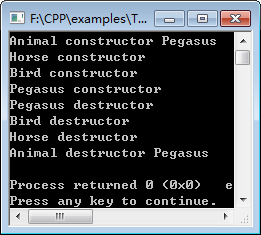
\includegraphics[width=0.3\textwidth]{figure/chap05/10-virtualctor}};
      
      \path let \p1=(fig) in
      coordinate (org) at (\x1, \y1)
      coordinate (ovBL1) at ($(org) + (-1.85, 1.03)$)
      coordinate (ovUR1) at ($(ovBL1) + (3.20, 0.22)$)
      ;

      \draw[red,thick,fill=green!25, fill opacity=0.14](ovBL1) rectangle
      (ovUR1);
      
    \end{tikzpicture}
  \end{center}
\end{frame}

\section[包含与继承]{包含与继承的选择}
\begin{frame}[t, fragile]{包含与继承}{包含与继承的选择}%
  \stretchon
  \begin{itemize}
  \item 接口的多继承有一定价值,但应避免实现多继承。在决定使用多继承之
    前,先仔细考虑其他替代方案。
  \item 继承是面向对象提供的另外一种复用代码的重要机制,继承使得派生类
    与基类之间具有接口的相似性。派生类可看作是基类的特定子类型,派生类
    对象可替代基类对象。
  \item 与包含相比,继承需要更多的技巧,而且易出错,包含是面向对象编程
    中的主要技术之一。
  \end{itemize}
  \stretchoff
\end{frame}

\begin{frame}[t, fragile]{包含与继承}{包含与继承的选择}%
  \stretchon
  \begin{itemize}  
  \item 何时使用继承,何时使用包含?
    \begin{itemize}
    \item 如果多个类共享数据而非行为,应该创建这些类可以包含的共用对象。
    \item 如果多个类共享行为而非数据,应该让它们从共同的基类继承而来,
      并在基类里定义共用的操作。
    \item 如果多个类既共享数据也共享行为,应该让它们从一个共同的基类继
      承而来,并在基类里定义共用的数据和操作。
    \item 如果想由基类控制接口,使用继承;如果想自己控制接口,使用包含。
    \end{itemize}
  \end{itemize}
  \stretchoff
\end{frame}
%%%%%%%%%%%%%%%%%%%%%%%%%%%%%%%%%%%%%%%%%%%%%%%%%%%%%%%%%%%%%%%%%%%%%%%%%%%%%%%

% 附件页
\section[附件下载]{本讲示例代码及附件下载} 
\begin{frame}{附件}{本讲附件}
  % 此处的[ucfilespec=...]必须指定为pdf否则Windows下无法下载
  %\vspace{-4ex}
  \textattachfile[ucfilespec=ex-src05.pdf]{ex-src05.zip}{附件:右键单击该
    链接,选择\qtmark{\alert{保存附件}}下载,\alert{将后缀名改为\qtmark{.zip}解压}
      \footnote[frame]{请\alert{退出全屏模式}后点击该链接。}
      \footnote[frame]{以Adobe Acrobat Reader为例。}
      。}%\\

  \vspace{-1ex}
  \begin{center}
    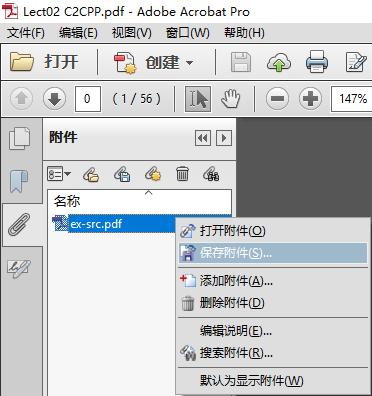
\includegraphics[height=0.35\textheight]{pdfattatchdownload01}\quad
    %或 \quad%
    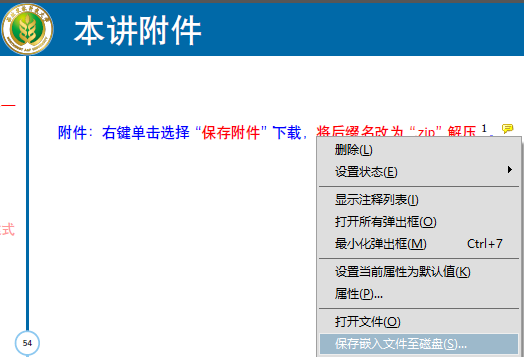
\includegraphics[height=0.35\textheight]{pdfattatchdownload02}\\[2ex]%
    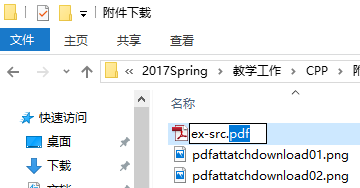
\includegraphics[height=0.255\textheight]{pdfattatchdownload03}\quad
    %$\Rightarrow$ \quad%
    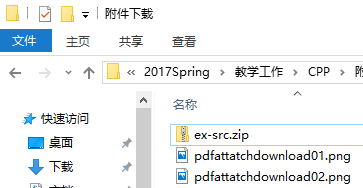
\includegraphics[height=0.255\textheight]{pdfattatchdownload04}%
  \end{center}   
\end{frame}


% \tiny
% \scriptsize
% \footnotesize
% \small
% \normalsize
% \large
% \Large
% \LARGE
% \huge
% \Huge


%%% Local Variables: 
%%% mode: latex
%%% TeX-master: "../main.tex"
%%% End: 
